\chapter{矢量与张量分析}

% ============================================================
\section{矢量代数}

设 $(x_1,x_2,x_3)$ 为三维空间中的点 $P$ 在右旋笛卡尔坐标系中的坐标（图 1）。
这些坐标唯一地确定了点 $P$ 在空间中的位置：$P:(x_1,x_2,x_3)$。
设 $(x_1',x_2',x_3')$ 为同一个点在另一个右旋笛卡尔坐标系中的坐标，则该点在两个不同的坐标系中的坐标由下式联系：

\begin{figure}[htbp]
\centering
\begin{tikzpicture}[tdplot_main_coords, scale=2.4]
  \coordinate (O) at (0,0,0);
  % 实线：原坐标系
  \draw[->,thick] (O) -- (2.1,0,0) node[anchor=north east]{$x_1(x)$};
  \draw[->,thick] (O) -- (0,2.1,0) node[anchor=north west]{$x_2(y)$};
  \draw[->,thick] (O) -- (0,0,2.1) node[anchor=south]{$x_3(z)$};
  % 虚线：旋转后的新坐标系
  \draw[->,dashed,thick] (O) -- (1.85,0.62,0.5) node[anchor=north east]{$x_1'$};
  \draw[->,dashed,thick] (O) -- (-0.52,1.8,0.5) node[anchor=north west]{$x_2'$};
  \draw[->,dashed,thick] (O) -- (-0.2,-0.4,1.95) node[anchor=south]{$x_3'$};
  % 点 P
  \coordinate (P) at (1.5,1.0,1.2);
  \fill (P) circle (1.2pt);
  \node[above right] at (P) {$P(x_1,x_2,x_3)$};
\end{tikzpicture}
\par\vspace{2pt}
{\small 图 1.}
\end{figure}

\begin{equation}
\begin{aligned}
x_1' &= u_{11} x_1 + u_{12} x_2 + u_{13} x_3,\\
x_2' &= u_{21} x_1 + u_{22} x_2 + u_{23} x_3,\\
x_3' &= u_{31} x_1 + u_{32} x_2 + u_{33} x_3,
\end{aligned}
\tag{1.1}
\end{equation}

式(1.1)可更紧凑地写成：

\begin{equation*}
x_i' = \sum_{j=1}^{3} u_{ij} x_j \qquad (i = 1, 2, 3).
\end{equation*}

显然，此时数 $u_{ij}$ 需服从下面的关系式：

\begin{equation}
\sum_{i=1}^{3} u_{ij} u_{ik} = \sum_{i=1}^{3} u_{ji} u_{ki} = \delta_{jk}
= \begin{cases} 1, & \text{若 } j = k,\\ 0, & \text{若 } j \neq k. \end{cases}
\tag{1.1a}
\end{equation}

[$\delta_{jk}$ 称为克罗内克（Kronecker）符号]

于是，
\begin{equation*}
\begin{aligned}
u_{11}^{2} + u_{21}^{2} + u_{31}^{2} &= 1,\\
u_{11} u_{12} + u_{21} u_{22} + u_{31} u_{32} &= 0,
\end{aligned}
\end{equation*}

等等。

由三个数组成的有序集合 $(A_1, A_2, A_3)$，在轴的旋转下能作象上述的点 $P$ 的坐标 $(x_1, x_2, x_3)$ 一样的变换，即
$(A_1, A_2, A_3) \longrightarrow (A_1', A_2', A_3')$，则 $(A_1, A_2, A_3)$ 就叫做三维矢量，这里

\begin{equation}
A_i' = \sum_{j=1}^{3} u_{ij} A_j \qquad (i = 1, 2, 3),
\tag{1.2}
\end{equation}

而 $u_{ij}$ 为 $(x_1, x_2, x_3)$ 变到 $(x_1', x_2', x_3')$ 时由(1.1)所确定的系数。

今考虑几个矢量的例子。空间中的点 $P(x_1, x_2, x_3)$ 可与具有同样坐标的矢量 $\ve{r}$ 相对应，这个矢量常称为 $P$ 点的径矢。如果矢量 $\ve{r}$ 依赖于某个变量 $t$，则我们可构成 $(dx_1/dt, dx_2/dt, dx_3/dt)$，容易验证，它也是矢量。这个矢量常记为 $\ve{v} = d\ve{r}/dt$。类似地，可构造矢量 $\ve{a} = d\ve{v}/dt$。一般地，如有某个坐标依赖于参数的矢量，则通过对原先的矢量按坐标微商可构造一新的矢量。用这种方法得到的矢量，就称为所给矢量的导数。

两个矢量 $\ve{A}$ 和 $\ve{B}$，只要在同一个坐标系中的对应坐标完全相同，就认为是相等的。显然，如果两个矢量在某一个坐标系中的坐标完全相同，那么它们在另外任意一个系中也完全相同。

矢量
\begin{equation*}
\ve{A} + \ve{B} = (A_1 + B_1,\ A_2 + B_2,\ A_3 + B_3)
\end{equation*}

称为两矢量 $\ve{A} = (A_1, A_2, A_3)$ 和 $\ve{B} = (B_1, B_2, B_3)$ 的和。容易检验，用这种方法得到的量确是一矢量，且

\begin{equation*}
\ve{A} + \ve{B} = \ve{B} + \ve{A}.
\end{equation*}

\textbf{例 1}\quad 矢量相等的几何解释。设 $\ve{A}$ 为某个矢量，而 $\ve{r}_P$，$\ve{r}_Q$ 分别为点 $P$ 和 $Q$ 的径矢。选取这样一些点，使得

\begin{equation*}
A_1 = x_{1P} - x_{1Q}, \qquad A_2 = x_{2P} - x_{2Q}, \qquad A_3 = x_{3P} - x_{3Q},
\end{equation*}

于是 $\ve{A} = \ve{r}_{PQ}$（图 3）。由此，任一矢量都可对应于某个线段；换句话说，所有矢量在空间中都有方向和大小这种特性。

\begin{figure}[htbp]
\centering
\begin{tikzpicture}[tdplot_main_coords, scale=2.2]
  \coordinate (O) at (0,0,0);
  % 坐标轴
  \draw[->,thick] (O) -- (2.1,0,0) node[anchor=north east]{$x_1$};
  \draw[->,thick] (O) -- (0,2.1,0) node[anchor=north west]{$x_2$};
  \draw[->,thick] (O) -- (0,0,2.1) node[anchor=south]{$x_3$};
  % 位置矢量 r → P
  \coordinate (P) at (1.5,1.0,1.2);
  \draw[->,very thick] (O) -- (P) node[midway,above]{$\ve{r}$};
  \fill (P) circle (1.2pt);
  \node[above] at (P) {$P(x_1,x_2,x_3)$};
\end{tikzpicture}
\par\vspace{2pt}
{\small 图 2.}
\end{figure}

\begin{figure}[htbp]
\centering
\begin{tikzpicture}[tdplot_main_coords, scale=2.2]
  \coordinate (O) at (0,0,0);
  % 坐标轴
  \draw[->,thick] (O) -- (2.1,0,0) node[anchor=north east]{$x_1$};
  \draw[->,thick] (O) -- (0,2.1,0) node[anchor=north west]{$x_2$};
  \draw[->,thick] (O) -- (0,0,2.1) node[anchor=south]{$x_3$};
  % 三角形 O-P-Q（原图三角形边无箭头；r_P 比 r_Q 长）
  \coordinate (P) at (1.5,1.1,1.7);
  \coordinate (Q) at (1.6,1.3,0.3);
  \draw[very thick] (O) -- (P) node[midway,below left]{$\ve{r}_P$};
  \draw[very thick] (O) -- (Q) node[midway,below right]{$\ve{r}_Q$};
  \draw[very thick] (P) -- (Q) node[midway,above right]{$\ve{r}_{PQ}$};
  \fill (O) circle (1.2pt);
  \fill (P) circle (1.2pt) node[above left]{$P$};
  \fill (Q) circle (1.2pt) node[below right]{$Q$};
\end{tikzpicture}
\par\vspace{2pt}
{\small 图 3.}
\end{figure}

数
\begin{equation*}
\ve{A} \cdot \ve{B} = \sum_{i=1}^{3} A_i B_i
\end{equation*}

称为两矢量 $\ve{A}$ 和 $\ve{B}$ 的数量积 $\ve{A} \cdot \ve{B}$。数量积是关于坐标系旋转的不变量。事实上，利用公式(1.1)得

\begin{equation*}
\begin{aligned}
\sum_{i=1}^{3} A_i' B_i'
&= \sum_{i,j,k} u_{ij} A_j\, u_{ik} B_k
 = \sum_{j,k} \left(\sum_{i=1}^{3} u_{ij} u_{ik}\right) A_j B_k\\
&= \sum_{j,k} \delta_{jk} A_j B_k = \sum_{j=1}^{3} A_j B_j.
\end{aligned}
\end{equation*}

在坐标系作转动时不变的量，叫做标量。于是 $\ve{A} \cdot \ve{B}$ 是标量。显然，$\ve{A} \cdot \ve{A} = \sum_{i=1}^{3} A_i^{2}$。数 $(\ve{A} \cdot \ve{A})^{1/2}$ 称为矢量 $\ve{A}$ 的模（或长度），并记之为 $|\ve{A}|$。特别是，如果 $\ve{A} = \ve{r}$，则

\begin{equation*}
|\ve{A}| = |\ve{r}| = \sqrt{x_1^{2} + x_2^{2} + x_3^{2}}.
\end{equation*}

今选取坐标系，使得轴 $x_1$ 顺着矢量 $\ve{A}$ 的方向，而矢量 $\ve{B}$ 则在平面 $x_1 x_2$ 内（图 4），于是

\begin{figure}[htbp]
\centering
\begin{tikzpicture}[scale=1.8]
  % x1 轴 = 矢量 A（同一条黑色带箭头线段）
  \draw[->,very thick] (-0.2,0) -- (3.6,0);
  \node[right] at (3.65,0) {$x_1$};
  \node[below] at (1.85,-0.14) {$A$};
  % x2 轴
  \draw[->] (0,-0.2) -- (0,2.5) node[above]{$x_2$};
  % 矢量 B（黑色带箭头）
  \draw[->,very thick] (0,0) -- (2.6,1.95) node[midway,above left]{$B$};
  % θ 弧（较大，离原点较远）
  \draw (1.12,0) arc[start angle=0, end angle=36.9, radius=1.12];
  \node at (1.52,0.42) {$\theta$};
\end{tikzpicture}
\par\vspace{2pt}
{\small 图 4.}
\end{figure}

\begin{equation*}
\begin{aligned}
\ve{A} &= (A, 0, 0),\\
\ve{B} &= (B \cos\theta,\ B \sin\theta,\ 0),\\
\ve{A} \cdot \ve{B} &= |\ve{A}|\,|\ve{B}| \cos\theta,
\end{aligned}
\end{equation*}

这里 $\theta$ 是矢量 $\ve{A}$ 和 $\ve{B}$ 之间的夹角。因 $\ve{A} \cdot \ve{B}$ 是标量，故这个等式在任意坐标系中都仍适合。特别地，如果 $\ve{A} \cdot \ve{B} = 0$，且 $\ve{A}$ 和 $\ve{B}$ 都不为零，则矢量 $\ve{A}$ 和 $\ve{B}$ 垂直。

\textbf{例 2}\quad 能量守恒。由牛顿第二定律

\begin{equation}
\ve{F} = m \ve{a} = m \frac{d\ve{v}}{dt},
\tag{1.3}
\end{equation}

这里 $m$ 为物体质量，$\ve{F}$ 为作用于该物体上的力，$\ve{v}$ 为速度。
在等式(1.3)两边点乘 $\ve{v}$，则得

\begin{equation*}
\begin{aligned}
\ve{F} \cdot \ve{v}
&= m \frac{d\ve{v}}{dt} \cdot \ve{v} = \sum_{i=1}^{3} m \frac{dv_i}{dt} v_i\\
&= \sum_{i=1}^{3} m \frac{d}{dt} \left(\frac{v_i^{2}}{2}\right) = \frac{d}{dt} \left(\frac{m v^{2}}{2}\right),
\end{aligned}
\end{equation*}

即
\begin{equation*}
\ve{F} \cdot \ve{v} = \frac{d}{dt} \left(\frac{m v^{2}}{2}\right)
\end{equation*}

这里 $v$ 为矢量 $\ve{v}$ 的模。特别，如果 $\ve{F} = 0$，则

\begin{equation*}
\frac{d}{dt} \left(\frac{m v^{2}}{2}\right) = 0, \qquad \text{即} \quad \frac{m v^{2}}{2} = \mathrm{const}.
\end{equation*}

这是能量守恒定律的一种形式。

\textbf{定理 1.1}\quad 假定有一个法则，使在每一坐标系中都能给出三个数 $(A_1, A_2, A_3)$，如果此法则对所有矢量 $\ve{B} = (B_1, B_2, B_3)$，都能使量 $\sum_{i=1}^{3} A_i B_i$ 为标量，则量 $\ve{A} = (A_1, A_2, A_3)$ 为矢量。

\textbf{证明}\quad 在坐标系转动下，矢量 $\ve{B}$ 的坐标按公式(1.2)变成：

\begin{equation*}
B_i' = \sum_{j=1}^{3} u_{ij} B_j \qquad (i = 1, 2, 3).
\end{equation*}

设在转动时，$(A_1, A_2, A_3)$ 变成 $(A_1', A_2', A_3')$。

我们需证
\begin{equation*}
A_i' = \sum_{j=1}^{3} u_{ij} A_j \qquad (i = 1, 2, 3).
\end{equation*}

但由假设
\begin{equation*}
\sum_{i=1}^{3} A_i' B_i' = \sum_{i=1}^{3} A_i B_i,
\end{equation*}

所以
\begin{equation*}
\sum_{i=1}^{3} A_i B_i = \sum_{i=1}^{3} A_i' \sum_{j=1}^{3} u_{ij} B_j = \sum_{j=1}^{3} \left(\sum_{i=1}^{3} u_{ij} A_i'\right) B_j.
\end{equation*}

因矢量 $\ve{B}$ 是任意给定的，故

\begin{equation}
A_j = \sum_{k=1}^{3} u_{kj} A_k' \qquad (j = 1, 2, 3).
\tag{1.4}
\end{equation}

将(1.4)乘以 $u_{ij}$，且对 $j$ 求和，考虑到(1.2)，就得

\begin{equation*}
\begin{aligned}
\sum_{j=1}^{3} u_{ij} A_j
&= \sum_{j=1}^{3} \sum_{k=1}^{3} u_{ij} u_{kj} A_k' = \sum_{k=1}^{3} A_k' \sum_{j=1}^{3} u_{ij} u_{kj}\\
&= \sum_{k=1}^{3} \delta_{ik} A_k' = A_i' \qquad (i = 1, 2, 3),
\end{aligned}
\end{equation*}

这就是所要证明的。

现考虑某个直角坐标系。设 $\ve{i} = (1, 0, 0)$，$\ve{j} = (0, 1, 0)$，$\ve{k} = (0, 0, 1)$ 为此坐标系中的三个单位矢量。则

\begin{equation*}
\begin{aligned}
\ve{i} \cdot \ve{i} = \ve{j} \cdot \ve{j} = \ve{k} \cdot \ve{k} &= 1,\\
\ve{i} \cdot \ve{j} = \ve{j} \cdot \ve{k} = \ve{k} \cdot \ve{i} &= 0
\end{aligned}
\end{equation*}

这些关系显示了单位矢量之间是相互垂直的。在这个坐标系中，矢量 $\ve{A} = (A_1, A_2, A_3)$ 可表示为

\begin{equation}
\ve{A} = A_1 \ve{i} + A_2 \ve{j} + A_3 \ve{k}.
\tag{1.5}
\end{equation}

将坐标轴旋转。原坐标系中的单位矢量在新坐标系中的坐标为

\begin{equation*}
\begin{aligned}
\ve{i} &: (u_{11}, u_{21}, u_{31}),\\
\ve{j} &: (u_{12}, u_{22}, u_{32}),\\
\ve{k} &: (u_{13}, u_{23}, u_{33}).
\end{aligned}
\end{equation*}

假定 $\ve{i}' = (1, 0, 0)$，$\ve{j}' = (0, 1, 0)$，$\ve{k}' = (0, 0, 1)$ 是新坐标系 $(x_1', x_2', x_3')$ 中的单位矢量。则由(1.2)和(1.5)式

\begin{equation}
\begin{aligned}
\ve{i} &= u_{11} \ve{i}' + u_{21} \ve{j}' + u_{31} \ve{k}',\\
\ve{j} &= u_{12} \ve{i}' + u_{22} \ve{j}' + u_{32} \ve{k}',\\
\ve{k} &= u_{13} \ve{i}' + u_{23} \ve{j}' + u_{33} \ve{k}'.
\end{aligned}
\tag{1.6}
\end{equation}

显然 $\ve{i}' \cdot \ve{i}' = 1$，$\ve{i}' \cdot \ve{j}' = 0$ 等等。因此

\begin{equation*}
\begin{aligned}
\ve{i} \cdot \ve{i} &= u_{11}^{2} + u_{21}^{2} + u_{31}^{2} = 1,\\
\ve{i} \cdot \ve{j} &= u_{11} u_{12} + u_{21} u_{22} + u_{31} u_{32} = 0.
\end{aligned}
\end{equation*}

我们又得到了(1.1)，并顺便说明了它们的起源。注意，由前面的结论从(1.4)式可推出，新坐标系中的单位矢量可用下面的方式由原坐标系中的单位矢量表出：

\begin{equation}
\begin{aligned}
\ve{i}' &= u_{11} \ve{i} + u_{12} \ve{j} + u_{13} \ve{k},\\
\ve{j}' &= u_{21} \ve{i} + u_{22} \ve{j} + u_{23} \ve{k},\\
\ve{k}' &= u_{31} \ve{i} + u_{32} \ve{j} + u_{33} \ve{k}.
\end{aligned}
\tag{1.7}
\end{equation}

有两个矢量 $\ve{A}$ 和 $\ve{B}$，若置

\begin{equation*}
\begin{aligned}
\ve{A} \times \ve{B} &= (A_2 B_3 - A_3 B_2,\ A_3 B_1 - A_1 B_3,\\
&\qquad\quad A_1 B_2 - A_2 B_1),
\end{aligned}
\end{equation*}

则可构造第三个矢量。下面将验证，$\ve{A} \times \ve{B}$ 确是矢量。为此，利用定理 1.1。即要证明，对所有矢量 $\ve{C}$，$(\ve{A} \times \ve{B}) \cdot \ve{C}$ 是标量。容易验证，

\begin{equation}
(\ve{A} \times \ve{B}) \cdot \ve{C} =
\begin{vmatrix}
A_1 & A_2 & A_3\\
B_1 & B_2 & B_3\\
C_1 & C_2 & C_3
\end{vmatrix}
\tag{1.8}
\end{equation}

位于(1.8)式右边的行列式，等于由矢量 $\ve{A}$，$\ve{B}$ 和 $\ve{C}$ 所构成的平行六面体的体积。显然，体积关于旋转是不变的。而这对

\begin{figure}[htbp]
\centering
\begin{tikzpicture}[scale=1.7]
  \coordinate (O) at (0,0);
  % A（黑色线段，无箭头，沿 i 方向=左下）
  \draw[very thick] (O) -- (-2.3,-1.15) node[midway,below left]{$A$};
  % B（黑色线段，无箭头，沿 j 方向=右）
  \draw[very thick] (O) -- (2.55,0) node[midway,below]{$B$};
  % A×B（黑色带箭头，沿 k 方向=上）
  \draw[->,very thick] (O) -- (0,2.45) node[midway,left]{$A \times B$};
  % 单位矢量 i、j、k 靠近原点
  \node[below left] at (-0.9,-0.45) {$i$};
  \node[below] at (0.8,0.2) {$j$};
  \node[above] at (0.18,0.8) {$k$};
  % θ 大弧（从 A 到 B，穿越 j 轴下方）
  \draw[->] (-0.95,-0.47) arc[start angle=-153.4, end angle=-12, radius=1.0];
  \node at (0.4,-0.95) {$\theta$};
  \fill (O) circle (1.2pt);
\end{tikzpicture}
\par\vspace{2pt}
{\small 图 5.}
\end{figure}

任一矢量 $\ve{C}$ 都是正确的，故由定理(1.1)知，$\ve{A} \times \ve{B}$ 确实是矢量。这个矢量称为矢量 $\ve{A}$ 和 $\ve{B}$ 的矢量积。

现在来确定矢量 $\ve{A} \times \ve{B}$ 的方向和大小。为此目的，我们选取坐标轴，使得矢量 $\ve{A}$ 顺着 $\ve{i}$ 的方向，而矢量 $\ve{B}$ 位于 $ij$ 平面内。于是在此坐标系内

\begin{equation*}
\ve{A} = (A, 0, 0),
\end{equation*}

\begin{equation*}
\ve{B} = (B \cos\theta,\ B \sin\theta,\ 0),
\end{equation*}

\begin{equation*}
\ve{A} \times \ve{B} = (0,\ 0,\ |\ve{A}|\,|\ve{B}| \sin\theta),
\end{equation*}

$\theta = \angle(\ve{A}, \ve{B})$ 为 $\ve{A}$ 和 $\ve{B}$ 之间的夹角。

因此
\begin{equation*}
|\ve{A} \times \ve{B}| = |\ve{A}|\,|\ve{B}|\,|\sin\theta|,
\end{equation*}

矢量 $\ve{A}$ 和 $\ve{B}$ 与矢量 $\ve{A} \times \ve{B}$ 垂直。矢量 $\ve{A}$，$\ve{B}$ 和 $\ve{A} \times \ve{B}$ 构成右旋三矢量。易知，如果矢量 $\ve{A}$ 与 $\ve{B}$ 平行，则 $\ve{A} \times \ve{B} = 0$；而在一般情形，矢量 $\ve{A} \times \ve{B}$ 的大小等于由矢量 $\ve{A}$ 和 $\ve{B}$ 所构成的平行四边形的面积。特别地，$\ve{i} \times \ve{i} = 0$ 等等，以及

\begin{equation*}
\ve{i} \times \ve{j} = \ve{k}, \qquad \ve{k} \times \ve{j} = -\ve{i}, \qquad \ve{j} \times \ve{k} = \ve{i}.
\end{equation*}

\textbf{例 3}\quad 有心力场内的动量矩守恒定律。设 $\ve{r} = \ve{r}(t)$ 为动点的径矢。如用 $\ve{F}$ 表示作用力，则由牛顿第二定律，$\ve{F} = m \ddot{\ve{r}}$（在矢量上面的点，今后都表示对时间 $t$ 的微商）。

如果矢量 $\ve{r}$ 和力 $\ve{F}$ 在任一时刻 $t$ 都互相平行，则力 $\ve{F}$ 称为有心力。重力，点电荷场内的静电力等都可以作为有心力的例子。要证明的是，在有心力的情形，矢量 $\ve{p} = m\ve{v}$（$\ve{p}$ 为动量，$m$ 为物体的质量，$\ve{v}$ 为物体的速度）常位于某个固定的平面内。今证明这个结论。

动点的径矢与其动量的矢量积叫做动量矩：

\begin{equation}
\ve{L} = \ve{r} \times \ve{p}.
\tag{1.9}
\end{equation}

(1.9)两边对 $t$ 微商，得

\begin{equation*}
\dot{\ve{L}} = \dot{\ve{r}} \times \ve{p} + \ve{r} \times \dot{\ve{p}}.
\end{equation*}

因动量矢与速度矢平行，故

\begin{equation*}
\dot{\ve{r}} \times \ve{p} = 0.
\end{equation*}

而由牛顿第二定律，$\dot{\ve{p}} = \ve{F}$；再由有心力的定义，便推得

\begin{equation*}
\ve{r} \times \dot{\ve{p}} = 0.
\end{equation*}

因此，
\begin{equation*}
\dot{\ve{L}} = 0 \qquad \text{或} \qquad \ve{L} = \mathrm{const}.
\end{equation*}

即在有心力的情形，动量矩是运动的积分（大小和方向守恒）。由(1.9)可看出，$\ve{p}$ 总位于与 $\ve{L}$ 垂直、在空间中位置固定的平面内。这就证明了我们的结论。

\textbf{例 4}\quad 无限小角度转动。考虑绕 $z$ 轴旋转。设 $\ve{r} = \ve{r}(t)$ 为质点在时刻 $t$ 的径矢，$\delta t$ 为无限小时间间隔。在 $\delta t$ 时间内，质点的径矢绕 $z$ 轴转过了小角度 $\delta\varphi$。因 $\delta\varphi \ll 1$，故下列关系式成立：

\begin{equation}
\cos\delta\varphi \approx 1 - \frac{(\delta\varphi)^{2}}{2}, \qquad
\sin\delta\varphi \approx \delta\varphi - \frac{(\delta\varphi)^{3}}{3!}.
\tag{1.10}
\end{equation}

利用(1.10)，可求出质点在转过 $\delta\varphi$ 角后（时间 $\delta t$ 后）的坐标：

\begin{equation}
\begin{aligned}
z(\delta t) &= z(0),\\
x(\delta t) &= x(0) - y(0)\,\delta\varphi + O(\delta\varphi^{2}),\\
y(\delta t) &= x(0)\,\delta\varphi + y(0) + O(\delta\varphi^{2}).
\end{aligned}
\tag{1.11}
\end{equation}

这里 $O(\delta\varphi^{2})$ 是 $(\delta\varphi)^{2}$ 的同级无穷小量。另一方面，当 $\delta t \to 0$ 时，在原点邻域内将 $x(t)$ 和 $y(t)$ 展开成泰勒（Taylor）级数，并限取前二项，则有

\begin{equation}
\begin{aligned}
x(\delta t) &= x(0) + \dot{x}\,\delta t,\\
y(\delta t) &= y(0) + \dot{y}\,\delta t.
\end{aligned}
\tag{1.12}
\end{equation}

比较(1.11)和(1.12)，就得

\begin{equation*}
\begin{aligned}
\dot{x}(t) &= -\left(\frac{\delta\varphi}{\delta t}\right) y,\\
\dot{y}(t) &= \left(\frac{\delta\varphi}{\delta t}\right) x,\\
\dot{z}(t) &= 0.
\end{aligned}
\end{equation*}

今用 $\ve{\omega}$ 记方向平行于旋转轴，大小等于 $\delta\varphi / \delta t$ 的矢量。在我们的情形，

\begin{equation*}
\ve{\omega} = \left(0,\ 0,\ \frac{\delta\varphi}{\delta t}\right)
\end{equation*}

因此
\begin{equation}
\dot{\ve{r}} = \ve{\omega} \times \ve{r}.
\tag{1.13}
\end{equation}

在(1.13)中所有的量都是矢量。因此，我们可以断言，这个等式在任一坐标系中都是正确的。

在 $\ve{\omega}$ 为常量的情形，加速度 $\ve{a}$ 可用下式计算：

\begin{equation*}
\begin{aligned}
\ve{a} \equiv \ddot{\ve{r}} &= \frac{d}{dt}(\ve{\omega} \times \ve{r}) = \ve{\omega} \times \dot{\ve{r}}\\
&= \ve{\omega} \times (\ve{\omega} \times \ve{r}),
\end{aligned}
\end{equation*}

如果矢量 $\ve{\omega}$ 与矢量 $\ve{r}$ 垂直，则

\begin{equation*}
|\ve{a}| = |\ve{\omega}|\,|\ve{\omega} \times \ve{r}| = |\ve{\omega}|^{2}\,|\ve{r}|,
\end{equation*}

且 $\ve{a}$ 与矢量 $\ve{r}$ 方向相反。而

\begin{equation*}
|\ve{v}| = |\ve{\omega} \times \ve{r}| = |\ve{\omega}|\,|\ve{r}|,
\end{equation*}

所以
\begin{equation*}
\ve{a} = -|\ve{\omega}|^{2}\,\ve{r} = -\frac{|\ve{v}|^{2}}{|\ve{r}|^{2}}\,\ve{r}.
\end{equation*}

现研究空间质点沿某个轨道运动的一般情形。假定

\begin{equation*}
\ve{\tau} = \frac{\ve{v}}{|\ve{v}|},
\end{equation*}

则 $\ve{\tau}$ 为与质点轨道相切的单位矢量（图 6）。将上式对 $t$ 微分，得

\begin{figure}[htbp]
\centering
\begin{tikzpicture}[tdplot_main_coords, scale=2.1]
  % 坐标轴
  \draw[->,thick] (0,0,0) -- (2.1,0,0) node[anchor=north east]{$x_1$};
  \draw[->,thick] (0,0,0) -- (0,2.1,0) node[anchor=north west]{$x_2$};
  \draw[->,thick] (0,0,0) -- (0,0,2.0) node[anchor=south]{$x_3$};
  % 空间曲线 r(t)（拱形，从左下向右上延伸）
  \draw[very thick] plot[smooth] coordinates
    {(0.55,0.35,0.08) (1.0,0.95,0.3) (1.5,1.65,0.55) (1.9,2.35,0.85) (2.1,3.0,1.15)};
  % 位置矢量 r（原点 → 曲线上的点 P）
  \coordinate (P) at (1.5,1.65,0.55);
  \draw[->,thick] (0,0,0) -- (P) node[midway,below right]{$\ve{r}$};
  \fill (P) circle (1.2pt);
  % Frenet 标架：τ 沿切线（右略上），N 竖直向上，b 右上方（原书为黑白）
  \draw[->,very thick] (P) -- +(0.35,0.65,0.35) node[above]{$\ve{\tau}$};
  \draw[->,very thick] (P) -- +(0,0,0.95) node[above]{$\ve{N}$};
  \draw[->,very thick] (P) -- +(0.25,0.5,0.6) node[right]{$\ve{b}$};
\end{tikzpicture}
\par\vspace{2pt}
{\small 图 6.}
\end{figure}

\begin{equation*}
\ve{a} \equiv \dot{\ve{v}} = \frac{d|\ve{v}|}{dt}\,\ve{\tau} + |\ve{v}|\, \dot{\ve{\tau}}.
\end{equation*}

但由等式 $\ve{\tau} \cdot \ve{\tau} = 1$ 推出

\begin{equation*}
\dot{\ve{\tau}} \cdot \ve{\tau} = 0,
\end{equation*}

即矢量 $\ve{\tau}$ 与 $\dot{\ve{\tau}}$ 垂直。这样一来，加速度 $\ve{a}$ 可分解为切向加速度和与它相垂直的法向加速度。引进单位矢量

\begin{equation}
\ve{N} = \frac{\dot{\ve{\tau}}}{|\dot{\ve{\tau}}|},
\tag{1.14}
\end{equation}

它与 $\ve{\tau}$ 垂直。并称它为曲线 $\ve{r} = \ve{r}(t)$ 的法矢量。如果 $S$ 为曲线从任一固定点量起的弧长，则下面等式成立：

\begin{equation}
\dot{\ve{\tau}} = \dot{S}\,\frac{d\ve{\tau}}{dS} = |\ve{v}|\,\frac{d\ve{\tau}}{dS}, \qquad (\dot{S} = |\ve{v}|)
\tag{1.15}
\end{equation}

由此
\begin{equation*}
\ve{N} = \frac{\dot{\ve{\tau}}}{|\ve{v}|\left|\frac{d\ve{\tau}}{dS}\right|},
\end{equation*}

\begin{equation*}
\ve{a} = \ve{N}\,|\ve{v}|^{2}\left|\frac{d\ve{\tau}}{dS}\right| + \ve{\tau}\,|\dot{\ve{v}}|.
\end{equation*}

量
\begin{equation*}
R \equiv \frac{1}{\left|\frac{d\ve{\tau}}{dS}\right|}
\end{equation*}

称为曲线的曲率半径。$R = \infty$（即 $d\ve{\tau}/dS = 0$）时的点称为曲线的拐点。

现在我们能写

\begin{equation*}
\ve{a} = \ve{N}\,\frac{|\ve{v}|^{2}}{R} + \ve{\tau}\,|\dot{\ve{v}}|.
\end{equation*}

对于匀速圆周运动，这个公式便成为

\begin{equation*}
\ve{a} = -\frac{|\ve{v}|^{2}}{|\ve{r}|^{2}}\,\ve{r}.
\end{equation*}

矢量 $\ve{N}$ 的方向用矢量 $d\ve{\tau}/dS$ 的方向确定。

根据定义，速度矢量 $\ve{v}$ 和加速度矢量 $\ve{a}$ 一样，位于由法向和切向单位矢量所构成的平面内。

因法向和切向单位矢量平面在空间中的位置随着时间而可能改变，于是速度和加速度给定了的质点轨道在一定程度上仍是自由的。我们将取曲线的挠率作为合适的参量。下面在计算自由加速度时，将利用挠率的概念。

法矢量和切矢量的矢量积 $\ve{b}$，叫做副法矢量：

\begin{equation}
\ve{b} = \ve{\tau} \times \ve{N}.
\tag{1.16}
\end{equation}

例如，若质点在平面内运动，则副法矢量为常量。

今用公式
\begin{equation*}
T \equiv \left|\frac{d\ve{b}}{dS}\right|
\end{equation*}

定义曲线的挠率 $T$。由图 7 看出，$|d\ve{b}| = d\theta$，因为 $|\ve{b}| = 1$，$\ve{b}$ 与矢量 $\ve{\tau}$ 与 $\ve{N}$ 的平面垂直以及 $d\theta$ 是这个平面的转动角。

\begin{figure}[htbp]
\centering
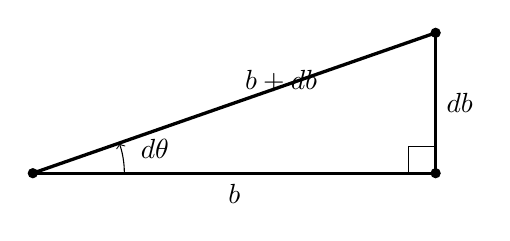
\begin{tikzpicture}[scale=1.55]
  % 直角三角形：底边 b、右边 db、斜边 b+db（说明 |db| = dθ）
  \coordinate (A) at (0,0);
  \coordinate (B) at (3.3,0);
  \coordinate (C) at (3.3,1.15);
  \draw[very thick] (A) -- (B) node[midway,below]{$b$};
  \draw[very thick] (B) -- (C) node[midway,right]{$db$};
  \draw[very thick] (A) -- (C) node[midway,above right]{$b+db$};
  \fill (A) circle (1.2pt) (B) circle (1.2pt) (C) circle (1.2pt);
  % dθ 弧（左下角）
  \draw[->] (0.75,0) arc[start angle=0, end angle=19.2, radius=0.75];
  \node at (1.0,0.2) {$d\theta$};
  % 直角标记
  \draw (3.08,0) -- (3.08,0.22) -- (3.3,0.22);
\end{tikzpicture}
\par\vspace{2pt}
{\small 图 7.}
\end{figure}

有时我们还用下面的记号：

\begin{equation*}
C_1 = \frac{1}{R} \text{——曲线曲率（第一曲率）},
\end{equation*}

\begin{equation*}
C_2 = \left|\frac{d\ve{b}}{dS}\right| \text{——曲线挠率（第二曲率）}, \qquad
C = \sqrt{C_1^{2} + C_2^{2}} \text{——全曲率}.
\end{equation*}

微分(1.16)，得

\begin{equation*}
\dot{\ve{b}} = \dot{\ve{\tau}} \times \ve{N} + \ve{\tau} \times \dot{\ve{N}}.
\end{equation*}

但矢量 $\dot{\ve{\tau}}$ 平行于矢量 $\ve{N}$，因此，$\dot{\ve{\tau}} \times \ve{N} = 0$，所以

\begin{equation*}
\dot{\ve{b}} = \ve{\tau} \times \dot{\ve{N}}.
\end{equation*}

因 $\ve{b} \cdot \ve{b} = 1$，故 $\dot{\ve{b}} \cdot \ve{b} = 0$。这样矢量 $\dot{\ve{b}}$ 就和矢量 $\ve{b}$ 与 $\ve{\tau}$ 垂直，从而就知矢量 $\dot{\ve{b}}$ 和矢量 $\ve{N}$ 平行。

\textbf{定理 1.2}\quad 全曲率等于矢量 $d\ve{N}/dS$ 的模：

\begin{equation*}
C = \left|\frac{d\ve{N}}{dS}\right|.
\end{equation*}

\textbf{证明}\quad 在矢量积(1.16)内进行循环交换，就给出

\begin{equation}
\ve{N} = \ve{b} \times \ve{\tau}.
\tag{1.17}
\end{equation}

将(1.17)对 $S$ 微分，得

\begin{equation}
\frac{d\ve{N}}{dS} = \frac{d\ve{b}}{dS} \times \ve{\tau} + \ve{b} \times \frac{d\ve{\tau}}{dS}.
\tag{1.18}
\end{equation}

其次，由(1.15)和(1.14)容易看出，矢量 $\ve{N}$ 平行于 $d\ve{\tau}/dS$，所以矢量 $\ve{b} \times d\ve{\tau}/dS$ 与矢量 $\dot{\ve{\tau}}$ 垂直。现在很明显，矢量 $\ve{b} \times d\ve{\tau}/dS$ 平行于矢量 $\ve{\tau}$。此外，

\begin{equation}
\left|\ve{b} \times \frac{d\ve{\tau}}{dS}\right| = \left|\frac{d\ve{\tau}}{dS}\right| = C_1;
\tag{1.19}
\end{equation}

类似地可证，矢量 $(d\ve{b}/dS) \times \ve{\tau}$ 平行于 $\ve{b}$，而

\begin{equation}
\left|\frac{d\ve{b}}{dS} \times \ve{\tau}\right| = \left|\frac{d\ve{b}}{dS}\right| = C_2.
\tag{1.20}
\end{equation}

在等式(1.18)右边部分内是两个互相垂直的矢量。因此，由(1.19)和(1.20)即可推得定理的结论：

\begin{equation*}
C = \left|\frac{d\ve{N}}{dS}\right|.
\end{equation*}

% ============================================================
\section{张量代数}

许多从物理观点来看非常重要的量，既不是矢量也不是标量。作为例子，我们引进与物体转动惯量有关的量 $x_i x_j$。当物体转动时，此量按下式变换：

\begin{equation*}
x_i' x_j' = \sum_{k,l=1}^{3} u_{ik} u_{jl}\, x_k x_l.
\end{equation*}

引入张量的概念。如果每个笛卡尔坐标系都有 $3^{n}$ 个数 $T_{i_1 i_2 \cdots i_n}$（这里 $i_1, i_2, \cdots, i_n$ 各自跑过值 $1, 2, 3$）与之对应，且这些数当由一个笛卡尔坐标系变到另一个时按规律

\begin{equation}
T_{i_1 i_2 \cdots i_n}' = \sum_{j_1, j_2, \cdots, j_n = 1}^{3} u_{i_1 j_1} u_{i_2 j_2} \cdots u_{i_n j_n}\, T_{j_1 j_2 \cdots j_n}
\tag{1.21}
\end{equation}

变换，则这 $3^{n}$ 个数全体就称为三维空间中的一个 $n$ 阶张量，这里 $u_{ij}$ 是过渡到新坐标系的矩阵。现考虑几个张量的例子。

\textbf{例 5}\quad $n = 1$。一阶张量有 $3^{1} = 3$ 个分量 $T_i\ (i = 1, 2, 3)$。它由公式

\begin{equation*}
T_i' = \sum_{j=1}^{3} u_{ij} T_j \qquad (i = 1, 2, 3)
\end{equation*}

进行变换。由此即知，一阶张量是矢量。

\textbf{例 6}\quad $n = 0$。推广张量的定义。零阶张量，它有一个分量 $S\ (3^{0} = 1)$，从一个笛卡尔坐标系变到另一个时，它不变：$S' = S$。

\textbf{例 7}\quad $n = 2$。二阶张量有 $3^{2} = 9$ 个分量。它们中的任一个都按下面的公式变换：

\begin{equation*}
T_{ij}' = \sum_{k=1}^{3} \sum_{l=1}^{3} u_{ik} u_{jl}\, T_{kl}.
\end{equation*}

如果一个张量的分量从一个坐标系过渡到另一个坐标系时不变，则这个张量就称为不变的。例如，$\delta_{ij}$ 就是一个二阶不变张量：

\begin{equation*}
\sum_{k,l=1}^{3} u_{ik} u_{jl}\, \delta_{kl} = \sum_{k=1}^{3} u_{ik} u_{jk} = \delta_{ij}.
\end{equation*}

\textbf{定理 1.3}\quad 如果 $T_{i_1 i_2 \cdots i_n}$ 是 $n$ 阶张量，则量

\begin{equation*}
H_{i_3 i_4 \cdots i_n} \equiv \sum_{i_1, i_2 = 1}^{3} \delta_{i_1 i_2}\, T_{i_1 i_2 \cdots i_n}
\end{equation*}

是 $n - 2$ 阶张量。

\textbf{证明}\quad 显然，量 $H_{i_3 i_4 \cdots i_n}$ 有 $3^{n-2}$ 个分量。要说明的是，在坐标系变换下，分量 $H_{i_3 i_4 \cdots i_n}$ 中的每一个是怎样改变的。

\begin{equation*}
\begin{aligned}
H_{i_3 i_4 \cdots i_n}' &= \sum_{i_1, i_2} \delta_{i_1 i_2}\, T_{i_1 i_2 \cdots i_n}'\\
&= \sum_{i_1, i_2} \sum_{j_1, \cdots, j_n} \delta_{i_1 i_2}\, u_{i_1 j_1} \cdots u_{i_n j_n}\, T_{j_1 j_2 \cdots j_n}\\
&= \sum_{j_1, \cdots, j_n} \left(\sum_{i_1 = 1}^{3} u_{i_1 j_1} u_{i_1 j_2}\right) u_{i_3 j_3} \cdots u_{i_n j_n}\, T_{j_1 j_2 \cdots j_n}.
\end{aligned}
\end{equation*}

其次，利用(1.1a)式，这一串等式可按下面的方式继续下去：

\begin{equation*}
= \sum_{j_3, \cdots, j_n} \left(\sum_{j_1, j_2} \delta_{j_1 j_2}\, T_{j_1 j_2 \cdots j_n}\right) u_{i_3 j_3} \cdots u_{i_n j_n}
= \sum_{j_3, \cdots, j_n} u_{i_3 j_3} \cdots u_{i_n j_n}\, H_{j_3 \cdots j_n}.
\end{equation*}

由此可见，量 $H_{i_3 i_4 \cdots i_n}$ 按(1.21)变化，即它是 $(n - 2)$ 阶张量。

\textbf{定理 1.4}\quad 若 $S_{i_1 i_2 \cdots i_n}$ 是 $n$ 阶张量的分量，$T_{j_1 j_2 \cdots j_m}$ 是 $m$ 阶张量的分量，则量

\begin{equation*}
S_{i_1 i_2 \cdots i_n}\, T_{j_1 j_2 \cdots j_m}
\end{equation*}

是 $(m + n)$ 阶张量的分量。

这个张量称为张量 $\ve{S}$ 和 $\ve{T}$ 的积。

\textbf{证明}\quad 所给张量的分量，在坐标系旋转时按下面的方式变换：

\begin{equation*}
S_{i_1 i_2 \cdots i_n}' = \sum_{k_1, k_2, \cdots, k_n} u_{i_1 k_1} u_{i_2 k_2} \cdots u_{i_n k_n}\, S_{k_1 k_2 \cdots k_n},
\end{equation*}

\begin{equation*}
T_{j_1 j_2 \cdots j_m}' = \sum_{l_1, l_2, \cdots, l_m} u_{j_1 l_1} u_{j_2 l_2} \cdots u_{j_m l_m}\, T_{l_1 l_2 \cdots l_m}.
\end{equation*}

因此量 $S_{i_1 i_2 \cdots i_n}\, T_{j_1 j_2 \cdots j_m}$ 和 $(m + n)$ 阶张量的分量一样地变换，即

\begin{equation*}
\begin{aligned}
&(S_{i_1 i_2 \cdots i_n}\, T_{j_1 j_2 \cdots j_m})'\\
&\quad = \sum_{k_1, \cdots, k_n} \sum_{l_1, \cdots, l_m} u_{i_1 k_1} \cdots u_{i_n k_n}\, u_{j_1 l_1} \cdots u_{j_m l_m}\, S_{k_1 \cdots k_n}\, T_{l_1 \cdots l_m}.
\end{aligned}
\end{equation*}

例如，如果 $A_i$ 和 $B_j$ 是矢量 $\ve{A}$ 和 $\ve{B}$ 的分量，则 $A_i B_j$ 就是二阶张量的分量。

现考虑量 $\delta_{ij} A_i B_j$。前面（定理 1.3）我们已指出，如果 $T_{i_1 i_2 \cdots i_n}$ 是 $n$ 阶张量，则量 $\sum_{i_1, i_2 = 1}^{3} \delta_{i_1 i_2} T_{i_1 i_2 \cdots i_n}$ 是 $(n - 2)$ 阶张量。由此推出量

\begin{equation*}
\sum_{i,j} \delta_{ij} A_i B_j = \sum_{i=1}^{3} A_i B_i = \ve{A} \cdot \ve{B}
\end{equation*}

是零阶张量，即标量。

将张量的分量乘以 $\delta_{i_1 i_2}$，然后对 $i_1$、$i_2$ 求和的运算，叫做张量的收缩。

这样，量 $T_{i_3 i_4 \cdots i_n} = \sum_{i_1, i_2 = 1}^{3} \delta_{i_1 i_2} T_{i_1 i_2 \cdots i_n}$ 是张量 $T_{i_1 i_2 \cdots i_n}$ 的收缩。张量可对其任意两个下标收缩。注意，一个 $n$ 阶张量按不同对的下标收缩，一般说来，得到的是不同的 $(n - 2)$ 阶张量。

特别，若
\begin{equation*}
T_{i_1 i_2 i_3} \equiv A_{i_1} B_{i_2} C_{i_3},
\end{equation*}

则
\begin{equation*}
\sum_{i_1, i_2 = 1}^{3} \delta_{i_1 i_2} T_{i_1 i_2 i_3} = (\ve{A} \cdot \ve{B})\, C_{i_3},
\end{equation*}

\begin{equation*}
\sum_{i_2, i_3 = 1}^{3} \delta_{i_2 i_3} T_{i_1 i_2 i_3} = A_{i_1}\, (\ve{B} \cdot \ve{C}).
\end{equation*}

收缩是张量分析中的基本运算之一。前已指出，$T_{ij} = \delta_{ij}$ 是二阶不变张量。现在我们研究三阶不变张量的一个重要例子。先引进下面的定义。

在排列 $(1, 2, 3)$ 中两个符号的位置对调，叫做对换。一个排列 $(i_1, i_2, i_3)$，如果需经偶数次对换才能变成排列 $(1, 2, 3)$，就称为偶排列，否则就称为奇排列。例如，

\[
(2, 1, 3) \text{——奇排列}, \qquad (2, 3, 1) \text{——偶排列}.
\]

现命
\begin{equation*}
\varepsilon_{ijk} =
\begin{cases}
1,  & \text{若 } (i, j, k) \text{ 为偶排列},\\
-1, & \text{若 } (i, j, k) \text{ 为奇排列},\\
0,  & \text{若 } i, j, k \text{ 并非都不同}.
\end{cases}
\end{equation*}

\textbf{定理 1.5}\quad 量 $\varepsilon_{ijk}$ 为三阶不变张量。

\textbf{证明}\quad 在坐标变换 $(x_1, x_2, x_3) \longrightarrow (x_1', x_2', x_3')$ 下，新坐标系的单位矢量 $\ve{i}'$，$\ve{j}'$，$\ve{k}'$ 可由公式(1.7)用原来坐标系的单位矢量 $\ve{i}$，$\ve{j}$，$\ve{k}$ 来表示。容易验证等式

\begin{equation}
\ve{i}' \cdot (\ve{j}' \times \ve{k}') =
\begin{vmatrix}
u_{11} & u_{12} & u_{13}\\
u_{21} & u_{22} & u_{23}\\
u_{31} & u_{32} & u_{33}
\end{vmatrix} = 1.
\tag{1.22}
\end{equation}

在等式(1.22)中交换矢量 $\ve{i}'$，$\ve{j}'$，$\ve{k}'$ 的位置，则得

\begin{equation}
\begin{vmatrix}
u_{i1} & u_{i2} & u_{i3}\\
u_{j1} & u_{j2} & u_{j3}\\
u_{k1} & u_{k2} & u_{k3}
\end{vmatrix} =
\begin{cases}
+1, & \text{若 } (i,j,k) \text{ 为 } (1,2,3) \text{ 的偶排列},\\
-1, & \text{若 } (i,j,k) \text{ 为 } (1,2,3) \text{ 的奇排列},\\
0,  & \text{在其余情形}.
\end{cases}
\tag{1.23}
\end{equation}

现作和式：
\begin{equation}
\sum_{l,m,n=1}^{3} u_{il} u_{jm} u_{kn}\, \varepsilon_{lmn}.
\tag{1.24}
\end{equation}

因在任意两个下标相同的情况下，$\varepsilon_{lmn} = 0$，故和式(1.24)由 6 项组成，同时，每一项都是矩阵

\begin{equation}
\begin{pmatrix}
u_{i1} & u_{i2} & u_{i3}\\
u_{j1} & u_{j2} & u_{j3}\\
u_{k1} & u_{k2} & u_{k3}
\end{pmatrix}
\tag{1.25}
\end{equation}

的不同行、不同列的三个元素的乘积，而被加项的符号和矩阵(1.25)的行列式的对应项符号相同。由公式(1.23)—(1.25)，就推出等式

\begin{equation*}
\varepsilon_{ijk}' =
\begin{cases}
+1, & \text{若 } (i,j,k) \text{ 为偶排列},\\
-1, & \text{若 } (i,j,k) \text{ 为奇排列},\\
0,  & \text{其余情形}.
\end{cases}
\end{equation*}

这就证明了定理。而张量 $\varepsilon_{ijk}$ 称为列维-齐维他（Levi-Civita）符号。

在下面的叙述中，凡有 $n$ 个指标跑遍 $1, 2, 3$ 的量，我们都认为是 $n$ 阶张量。

\textbf{例 8}

a) $A_i B_j$——二阶张量；

b) $\varepsilon_{ijk} A_l B_m$——五阶张量；

c) $\sum_{j,k} \varepsilon_{ijk} A_j B_k = (A_2 B_3 - A_3 B_2) = (\ve{A} \times \ve{B})_i$——一阶张量；

d) $\sum_{i,j,k} \varepsilon_{ijk} T_{ijk}$——零阶张量（标量）。

若 $T_{ij} = T_{ji}$，则量 $T_{ij}$ 称为二阶对称张量。而如果 $T_{ij} = -T_{ji}$，则 $T_{ij}$ 称为二阶反对称张量。

例如，置 $S_{ij} = \sum_{k=1}^{3} \varepsilon_{ijk} A_k$，这里 $\ve{A}$ 为任一矢量，则由 $\varepsilon_{ijk}$ 的性质，$S_{ij} = -S_{ji}$。

\textbf{定理 1.6}\quad 张量的对称性（反对称性）是不变的。即对称（或反对称）张量在任何坐标系中都保持其对称（反对称）性。

\textbf{证明}\quad 设

\begin{equation}
T_{ij}' = \sum_{k,l} u_{ik} u_{jl}\, T_{kl},
\tag{1.26}
\end{equation}

\begin{equation}
T_{ji}' = \sum_{k,l} u_{jk} u_{il}\, T_{lk}.
\tag{1.27}
\end{equation}

在反对称张量的情形将(1.26)和(1.27)相加（在对称情形相减）：

\begin{equation}
T_{ij}' \pm T_{ji}' = \sum_{k,l} u_{ik} u_{jl}\, (T_{kl} \pm T_{lk}).
\tag{1.28}
\end{equation}

显然，等式(1.28)的右端恒等于零，于是左端也恒等于零。此事本身就证明了，张量的对称性（反对称性）在任一坐标系中都保持不变。

% ============================================================
\section{二阶张量的几何表示法}

\textbf{1. 反对称张量}\quad 因 $T_{ij} = -T_{ji}$，故由等式 $T_{ii} = -T_{ii}$ 推出

\begin{equation*}
T_{11} = T_{22} = T_{33} = 0,
\end{equation*}

而对张量的非对角分量有：

\begin{equation*}
T_{12} = -T_{21}, \qquad T_{13} = -T_{31}, \qquad T_{23} = -T_{32}.
\end{equation*}

由此，一个反对称张量完全由三个独立的量 $\{T_{12}, T_{13}, T_{23}\}$ 所确定。因此，很自然地就把它与某个矢量联系起来。反之，一坐标为 $A_k$ 的矢量 $\ve{A}$，可构造反对称张量

\begin{equation*}
T_{ij} = \frac{1}{2} \sum_{k} \varepsilon_{ijk} A_k,
\end{equation*}

这里 $\varepsilon_{ijk}$ 和前面的意义相同。

\textbf{2. 对称张量}\quad 因在此时 $T_{ij} = T_{ji}$，故张量 $T_{ij}$ 共有 6 个独立的分量：$T_{11}, T_{22}, T_{33}, T_{12}, T_{13}, T_{23}$。

这样的张量已不可能用矢量来表示，但我们可利用二阶曲面的性质。大家知道，二阶曲面是由 6 个独立的参数决定的，它的方程可写为

\begin{equation*}
A x^{2} + B y^{2} + C z^{2} + D xy + E xz + E' yz = 1.
\end{equation*}

\textbf{定理 1.7}\quad 任一非零二阶对称张量都唯一地对应了由下面方程所确定的二阶曲面：

\begin{equation}
\sum_{i,j} T_{ij}\, x_i x_j = \pm 1.
\tag{1.29}
\end{equation}

\textbf{附注：}右边的符号与由张量的分量 $T_{ij}$ 所组成的行列式的符号相一致（稍后我们将指出，若 $\det|T_{ij}| = 0$，则张量 $T_{ij}$ 恒等于零）。量 $\det|T_{ij}|$ 可表示为

\begin{equation}
\begin{aligned}
\det|T_{ij}| &=
\begin{vmatrix}
T_{11} & T_{12} & T_{13}\\
T_{21} & T_{22} & T_{23}\\
T_{31} & T_{32} & T_{33}
\end{vmatrix}\\
&= \frac{1}{6} \sum \varepsilon_{ijk}\, \varepsilon_{lmn}\, T_{il} T_{jm} T_{kn},
\end{aligned}
\tag{1.29a}
\end{equation}

因此，它是标量。符号规则是必须引进的，否则就会推出如下的关系式：$T_{ij} = -\delta_{ij}$ 和 $-x^{2} - y^{2} - z^{2} = 1$。而这在实空间内是不可能的。现转到定理的证明。

\textbf{证明}\quad 现证明方程(1.29)关于坐标旋转不变，即

\begin{equation*}
\sum_{i,j} T_{ij}'\, x_i' x_j' = \pm 1.
\end{equation*}

我们有：
\begin{equation*}
\begin{aligned}
\sum_{i,j} T_{ij}'\, x_i' x_j'
&= \sum_{i,j} \sum_{k,l} u_{ik} u_{jl}\, T_{kl} \sum_{m,n} u_{im} u_{jn}\, x_m x_n\\
&= \sum_{k,l,m,n} \left(\sum_{i} u_{ik} u_{im}\right) \left(\sum_{j} u_{jl} u_{jn}\right) T_{kl}\, x_m x_n\\
&= \sum_{k,l,m,n} \delta_{km}\, \delta_{ln}\, T_{kl}\, x_m x_n = \sum_{k,l} T_{kl}\, x_k x_l.
\end{aligned}
\end{equation*}

曲面方程的不变性和(1.29a)式即证明了定理。

\textbf{3. 二阶任意张量}\quad 二阶任意张量 $R_{ij}$ 可唯一地表示成对称和反对称张量之和：

\begin{equation*}
R_{ij} = S_{ij} + T_{ij},
\end{equation*}

这里 $S_{ij} = \frac{1}{2}(R_{ij} - R_{ji})$ 是反对称张量，$T_{ij} = \frac{1}{2}(R_{ij} + R_{ji})$ 是对称张量。

\textbf{例 9}\quad 惯性张量。刚体运动时，动量矩等于

\begin{equation*}
\ve{L} = \int (\ve{r} \times \ve{v})\, \rho\, d\tau.
\end{equation*}

在刚体转动时，利用(1.13)式，有

\begin{equation*}
\begin{aligned}
\ve{L} &= \int \rho\, d\tau\, [\ve{r} \times (\ve{\omega} \times \ve{r})]\\
&= \int \rho\, d\tau\, [\ve{\omega}\,|\ve{r}|^{2} - \ve{r}\,(\ve{\omega} \cdot \ve{r})].
\end{aligned}
\end{equation*}

量
\begin{equation*}
I_{ij} \equiv \int \rho\, [|\ve{r}|^{2}\, \delta_{ij} - r_i r_j]\, d\tau = I_{ji} \qquad (i, j = 1, 2, 3)
\end{equation*}

叫做惯性张量。于是

\begin{equation*}
\sum_{j=1}^{3} I_{ij}\, \omega_j = \int \rho\, d\tau \left[|\ve{r}|^{2}\, \omega_i - \left(\sum_{j} r_j \omega_j\right) r_i\right] \equiv L_i,
\end{equation*}

这里 $L_i$ 是动量矩在第 $i$ 坐标轴上的投影。在一般情况下，矢量 $\ve{L}$ 与 $\ve{\omega}$ 互不平行。在没有外力矩时，$\dot{\ve{L}} = 0$。因此矢量 $\ve{L}$ 固定，而矢量 $\ve{\omega}$ 绕矢量 $\ve{L}$ 旋进。假定关于某轴的转动惯量用公式

\begin{equation*}
J \equiv \int \rho\, S^{2}\, d\tau
\end{equation*}

表出，这里 $S$ 为到旋转轴的距离。特别，若绕 $z$ 轴，则 $S^{2} = x^{2} + y^{2}$。于是成立如下定理。

\textbf{定理 1.8}\quad 若 $l_i\ (i = 1, 2, 3)$ 为某个轴的方向余弦，则关于此轴的转动惯量等于

\begin{equation*}
J = \sum_{i,j=1}^{3} l_i\, I_{ij}\, l_j.
\end{equation*}

\textbf{证明}\quad 量 $\sum_{i,j} l_i I_{ij} l_j$ 为标量，故可在任一坐标系中来计算它。设所考虑的轴为 $z$ 轴，则 $(l_1, l_2, l_3)$ 变为 $(0, 0, 1)$，得

\begin{equation*}
\begin{aligned}
\sum_{i,j} l_i I_{ij} l_j &= I_{33} = \int \rho\, (|\ve{r}|^{2} - z^{2})\, d\tau\\
&= \int \rho\, (x^{2} + y^{2})\, d\tau = \int \rho\, S^{2}\, d\tau
\end{aligned}
\end{equation*}

这就是所要证明的。

% ============================================================
\section{张量场}

若 $3^{n}$ 个函数 $T_{i_1 i_2 \cdots i_n}(x_1, x_2, x_3)$ 在空间 $(x_1, x_2, x_3)$ 中的任一点处都成一张量，则这个 $3^{n}$ 个函数的全体就称为 $n$ 阶张量场。

\textbf{1. $n = 0$ 的情形}\quad 为标量场，即坐标的函数 $\Phi(\ve{r})$。

\textbf{例 10}\quad 点电荷势

\begin{equation*}
V(\ve{r}) = \frac{e}{|\ve{r}|}.
\end{equation*}

量
\begin{equation*}
|\ve{r}| = \left(\sum_{i=1}^{3} x_i^{2}\right)^{1/2}
\end{equation*}

是标量，故 $\Phi(\ve{r})$ 关于旋转不变。

\textbf{2. $n = 1$ 的情形}\quad 矢量场 $\ve{A}(\ve{r})$——以矢量为自变量的矢量函数。

\textbf{例 11}\quad 点电荷场

\begin{equation*}
\ve{E} = \frac{e}{|\ve{r}|^{3}}\, \ve{r}.
\end{equation*}

\textbf{定理 1.9}\quad 若 $T_{i_1 i_2 \cdots i_n}(\ve{r})$ 是 $n$ 阶张量场，则量 $\frac{\partial}{\partial x_i} T_{i_1 i_2 \cdots i_n}$ 是 $(n + 1)$ 阶张量场。

\textbf{证明}\quad 首先注意，在转动 $x_i' = \sum_{j=1}^{3} u_{ij} x_j$ 下，

\begin{equation*}
\left(\frac{\partial}{\partial x_i} T_{i_1 i_2 \cdots i_n}\right)' = \frac{\partial}{\partial x_i'} T_{i_1 i_2 \cdots i_n}'.
\end{equation*}

由条件(1.1a)推出，

\begin{equation*}
x_j = \sum_{i=1}^{3} u_{ij}\, x_i' \qquad \text{或} \quad \frac{\partial x_j}{\partial x_i'} = u_{ij}.
\end{equation*}

因此，
\begin{equation}
\frac{\partial}{\partial x_i'} = \sum_{j=1}^{3} \frac{\partial x_j}{\partial x_i'}\, \frac{\partial}{\partial x_j} = \sum_{j=1}^{3} u_{ij}\, \frac{\partial}{\partial x_j}
\tag{1.30}
\end{equation}

[在等式(1.30)中，假定所有 $x_j'\ (j \neq i)$ 和 $x_i\ (i \neq j)$ 都是固定的] 现在很清楚，量 $\frac{\partial}{\partial x_i} T_{i_1 i_2 \cdots i_n}$ 象 $(n + 1)$ 阶张量那样变换，即

\begin{equation*}
\frac{\partial}{\partial x_i'} T_{i_1 i_2 \cdots i_n}' = \sum_{j, j_1, \cdots, j_n} u_{ij}\, u_{i_1 j_1} \cdots u_{i_n j_n}\, \frac{\partial}{\partial x_j} T_{j_1 j_2 \cdots j_n},
\end{equation*}

而这种形式的分量个数等于 $3^{n+1}$。这样，定理便得证。

现考虑由此定理得出的几个推论：

\textbf{推论 1}\quad 如果 $\Phi(\ve{r})$ 是标量，则 $\frac{\partial\Phi}{\partial x_i}$ 是矢量的分量（$i = 1, 2, 3$），这个矢量称为场 $\Phi(\ve{r})$ 的梯度，它的分量一般记作

\begin{equation*}
(\nabla\Phi)_i \equiv \frac{\partial\Phi}{\partial x_i} \equiv [\operatorname{grad}\Phi]_i.
\end{equation*}

算子 $\nabla$ 称为梯度算子（“纳伯拉”）。

\textbf{推论 2}\quad 如果 $\ve{A}$ 为矢量，则 $\sum_{i=1}^{3} \frac{\partial A_i}{\partial x_i}$ 是标量，它称为矢量 $\ve{A}$ 的散度，且记为

\begin{equation*}
\nabla \cdot \ve{A} \equiv \operatorname{div}\ve{A}.
\end{equation*}

\textbf{推论 3}\quad 量

\begin{equation*}
\sum_{j,k} \varepsilon_{ijk}\, \frac{\partial A_k}{\partial x_j} \equiv (\nabla \times \ve{A})_i \equiv (\operatorname{rot}\ve{A})_i, \qquad (i = 1, 2, 3)
\end{equation*}

是矢量的分量。矢量 $\nabla \times \ve{A}$ 常称为旋度或涡度。

\textbf{推论 4}\quad 量

\begin{equation*}
\sum_{i=1}^{3} \frac{\partial^{2}\Phi}{\partial x_i^{2}} \equiv \triangle\Phi \equiv \nabla^{2}\Phi
\end{equation*}

是标量，这个标量称为标量函数 $\Phi$ 的拉普拉斯（Laplace）。

\textbf{推论 5}\quad 量

\begin{equation*}
\sum_{j=1}^{3} \frac{\partial^{2}}{\partial x_j^{2}} A_i \equiv (\triangle\ve{A})_i \equiv (\nabla^{2}\ve{A})_i
\end{equation*}

是矢量分量，叫做矢量函数 $\ve{A}$ 的拉普拉斯。

今证明与上述诸量有关的几个恒等式的正确性。

\textbf{恒等式 1}\quad 对任意 $\ve{A}$，

\begin{equation}
\nabla \cdot (\nabla \times \ve{A}) = 0.
\tag{1.31}
\end{equation}

\textbf{证明}\quad 我们有

\begin{equation*}
\begin{aligned}
\sum_{i,j,k} \frac{\partial}{\partial x_i}\, \varepsilon_{ijk}\, \frac{\partial A_k}{\partial x_j}
&= -\sum_{i,j,k} \varepsilon_{jik}\, \frac{\partial^{2} A_k}{\partial x_i \partial x_j}\\
&= -\sum_{i,j,k} \varepsilon_{jik}\, \frac{\partial^{2} A_k}{\partial x_j \partial x_i}.
\end{aligned}
\end{equation*}

再改变求和下标，得

\begin{equation*}
-\sum_{i,j,k} \varepsilon_{jik}\, \frac{\partial^{2} A_k}{\partial x_j \partial x_i}
= -\sum_{i,j,k} \varepsilon_{ijk}\, \frac{\partial^{2} A_k}{\partial x_i \partial x_j},
\end{equation*}

证毕。

\textbf{恒等式 2}\quad 对任意的 $\Phi$

\begin{equation}
\nabla \times (\nabla\Phi) = 0.
\tag{1.32}
\end{equation}

\textbf{证明}\quad 和前面相类似，

\begin{equation*}
\begin{aligned}
[\nabla \times (\nabla\Phi)]_i &= \sum_{j,k} \varepsilon_{ijk}\, \frac{\partial}{\partial x_j}\, \frac{\partial\Phi}{\partial x_k}\\
&= \sum_{j,k} \varepsilon_{ijk}\, \frac{\partial^{2}\Phi}{\partial x_j \partial x_k}
 = -\sum_{j,k} \varepsilon_{ikj}\, \frac{\partial^{2}\Phi}{\partial x_j \partial x_k}\\
&= -\sum_{j,k} \varepsilon_{ijk}\, \frac{\partial^{2}\Phi}{\partial x_k \partial x_j} = 0
\end{aligned}
\end{equation*}

\textbf{恒等式 3}\quad

\begin{equation}
\nabla \times (\nabla \times \ve{A}) = \nabla(\nabla \cdot \ve{A}) - \nabla^{2}\ve{A}.
\tag{1.33}
\end{equation}

\textbf{证明}\quad

\begin{equation*}
\begin{aligned}
[\nabla \times (\nabla \times \ve{A})]_i &= \sum_{j,k} \varepsilon_{ijk}\, \frac{\partial}{\partial x_j} (\nabla \times \ve{A})_k\\
&= \sum_{j,k,l,m} \varepsilon_{ijk}\, \varepsilon_{klm}\, \frac{\partial^{2} A_m}{\partial x_j \partial x_l}.
\end{aligned}
\end{equation*}

但
\begin{equation*}
\begin{aligned}
\varepsilon_{lmk} &= \varepsilon_{klm},\\
\sum_{k} \varepsilon_{ijk}\, \varepsilon_{klm} &= \delta_{il}\, \delta_{jm} - \delta_{im}\, \delta_{jl},
\end{aligned}
\end{equation*}

因此
\begin{equation*}
\begin{aligned}
[\nabla \times (\nabla \times \ve{A})]_i
&= \sum_{j,l,m} (\delta_{il}\, \delta_{jm} - \delta_{im}\, \delta_{jl})\, \frac{\partial^{2} A_m}{\partial x_j \partial x_l}\\
&= \sum_{m} \frac{\partial}{\partial x_m}\, \frac{\partial A_m}{\partial x_i} - \sum_{l} \frac{\partial^{2} A_i}{\partial x_l^{2}}.
\end{aligned}
\end{equation*}

显然
\begin{equation*}
[\nabla \times (\nabla \times \ve{A})]_i = \frac{\partial}{\partial x_i} (\nabla \cdot \ve{A}) - \nabla^{2} A_i,
\end{equation*}

这就证明了恒等式(1.33)。

现讨论梯度的几何解释和物理意义。方程 $\Phi(x, y, z) = \text{const}$ 是标量场 $\Phi(x, y, z)$ 的等位面。在原点的点电荷的场的等电位面，可作为等位面的一个物理例子。不难看出，这种曲面将是球面，因为

\begin{equation*}
\Phi(\ve{r}) = \frac{e}{|\ve{r}|}.
\end{equation*}

设 $\ve{E}$ 是矢量场（力场），若曲线上任意一点 $(x, y, z)$ 处的切线方向都与 $\ve{E}$ 在该点处的方向一致，则此曲线称为力线。力线的无限小线素用 $d\ve{s}$ 表示。由力线的这个定义推出

\begin{equation*}
\frac{dx_1}{E_1} = \frac{dx_2}{E_2} = \frac{dx_3}{E_3}.
\end{equation*}

通常力场用正交曲线网的图象来表示。为了作图，可先画出等位面，而力线沿着它的法向，同时力线的密度（在等位面的单位面积上的力线数目）用下面规则来确定：

\begin{equation*}
\frac{\text{力线的数目}}{(\text{法向的})\ \text{面积}} = |\ve{E}|.
\end{equation*}

为了解释这种作图方法的理由，尚需证明：力线正交于场 $\ve{E} = -\nabla\Phi$ 的等位面。取 $d\ve{s}$ 为曲面 $\Phi = \Phi_0$ 的无限小元素，则

\begin{equation*}
d\Phi = \nabla\Phi \cdot d\ve{s} = -\ve{E} \cdot d\ve{s} = 0.
\end{equation*}

显然，$\ve{E} \perp d\ve{s}$。这就是所要证明的。

\textbf{例 12}\quad 在坐标原点的点电荷的静电场为

\begin{equation*}
\Phi = \frac{e}{|\ve{r}|}.
\end{equation*}

它的梯度等于

\begin{equation*}
\begin{aligned}
\nabla\Phi &= -\frac{e}{|\ve{r}|^{3}}\, \ve{r} = -\ve{E}.
\end{aligned}
\end{equation*}

在两个点电荷系情形，它的等位面和力线如图 8 所示。

\begin{figure}[htbp]
\centering
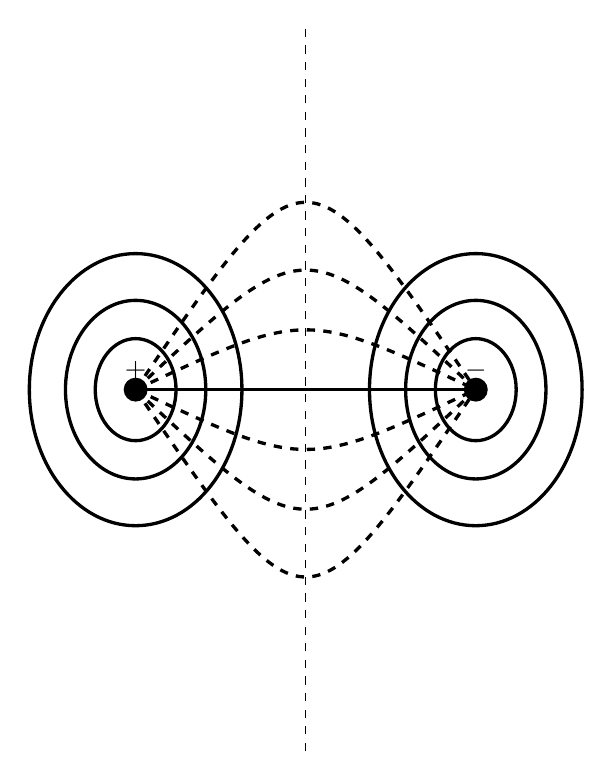
\begin{tikzpicture}[scale=1.35]
  % 电荷：+ 左、- 右
  \fill (-1.6,0) circle (3.2pt);
  \fill (1.6,0) circle (3.2pt);
  \node[above] at (-1.6,0) {$+$};
  \node[above] at (1.6,0) {$-$};
  % 实线：连接两电荷的水平线
  \draw[very thick] (-1.6,0) -- (1.6,0);
  % 实线：电荷周围的闭合等位线（各 3 层）
  \foreach \rx/\ry in {0.38/0.48, 0.66/0.84, 1.0/1.28} {
    \draw[very thick] (-1.6,0) ellipse ({\rx} and {\ry});
    \draw[very thick] (1.6,0) ellipse ({\rx} and {\ry});
  }
  % 虚线：从 + 到 - 的电场线（上下各 3 条弧）
  \foreach \h in {0.75,1.5,2.35} {
    \draw[dashed,very thick] (-1.6,0) .. controls (0,\h) .. (1.6,0);
    \draw[dashed,very thick] (-1.6,0) .. controls (0,-\h) .. (1.6,0);
  }
  % 虚线：竖直中垂线（零等位面），向两端延伸
  \draw[dashed] (0,-3.4) -- (0,3.4);
\end{tikzpicture}
\par\vspace{2pt}
{\small 图 8.}
\end{figure}

% ============================================================
\section{高斯-奥斯特洛格拉德斯基定理及其应用}

我们现在所要讲的定理，是矢量分析中最重要的定理之一。它把 $n$ 阶光滑张量场的面积分与 $(n + 1)$ 阶张量场的体积分联系了起来。

\textbf{定理 1.10}\quad 设给定了光滑张量场 $T_{i_1 i_2 \cdots i_n}(x_1, x_2, x_3)$，则下面的等式成立：

\begin{equation}
\sum_{i_1 = 1}^{3} \int_{V} \frac{\partial}{\partial x_{i_1}} T_{i_1 i_2 \cdots i_n}\, d\tau
= \int_{S} \sum_{i_1 = 1}^{3} T_{i_1 i_2 \cdots i_n}\, dS_{i_1},
\tag{1.34}
\end{equation}

这里 $d\tau$ 是体积元素，$d\ve{S}(dS_1, dS_2, dS_3)$ 为沿着曲面的外法线方向、长度在数值上等于曲面 $S$ 的面积元素的面积的矢量。

\textbf{证明}\quad 考虑任一由封闭曲面 $S$ 所围成的体积 $V$。将这个体积分割为若干个体积元素，使每个体积元素用立方体来逼近时达到给定的精确度。现对棱平行于坐标轴的立方体来证明公式(1.34)。位于等式(1.34)左边的积分，对于立方体可改写成下面的形状：

\begin{equation}
\begin{aligned}
&\int \frac{\partial}{\partial x_1} T_{1 i_2 i_3 \cdots i_n}\, dx_1 dx_2 dx_3
 + \int \frac{\partial}{\partial x_2} T_{2 i_2 i_3 \cdots i_n}\, dx_1 dx_2 dx_3\\
&\qquad + \int \frac{\partial}{\partial x_3} T_{3 i_2 i_3 \cdots i_n}\, dx_1 dx_2 dx_3\\
&= \int T_{1 i_2 i_3 \cdots i_n} \Big|_{x_1}^{x_1 + dx_1} dx_2 dx_3
 + \int T_{2 i_2 i_3 \cdots i_n} \Big|_{x_2}^{x_2 + dx_2} dx_1 dx_3\\
&\qquad + \int T_{3 i_2 i_3 \cdots i_n} \Big|_{x_3}^{x_3 + dx_3} dx_1 dx_2.
\end{aligned}
\tag{1.35}
\end{equation}

由图 9，显然

\begin{figure}[htbp]
\centering
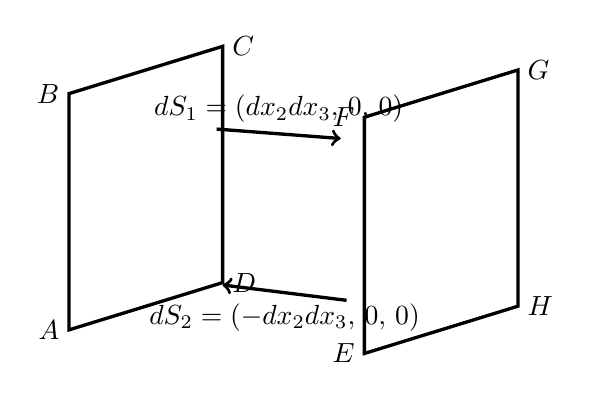
\begin{tikzpicture}[scale=1.5]
  % 左平面 ABCD（平行四边形）
  \coordinate (A) at (0.7,0.8);
  \coordinate (B) at (0.7,2.8);
  \coordinate (C) at (2.0,3.2);
  \coordinate (D) at (2.0,1.2);
  \draw[very thick] (A) -- (B) -- (C) -- (D) -- cycle;
  % 右平面 EFGH
  \coordinate (E) at (3.2,0.6);
  \coordinate (F) at (3.2,2.6);
  \coordinate (G) at (4.5,3.0);
  \coordinate (H) at (4.5,1.0);
  \draw[very thick] (E) -- (F) -- (G) -- (H) -- cycle;
  % 顶点标注
  \node[left]  at (A) {$A$};
  \node[left]  at (B) {$B$};
  \node[right] at (C) {$C$};
  \node[right] at (D) {$D$};
  \node[left]  at (E) {$E$};
  \node[left]  at (F) {$F$};
  \node[right] at (G) {$G$};
  \node[right] at (H) {$H$};
  % 面积元箭头：上（右向）、下（左向），从平面内部出发、到达另一平面
  \draw[->,very thick] (1.95,2.5) -- (3.0,2.42) node[midway,above]{$d\ve{S}_1 = (dx_2 dx_3,\,0,\,0)$};
  \draw[->,very thick] (3.05,1.05) -- (2.0,1.18) node[midway,below]{$d\ve{S}_2 = (-dx_2 dx_3,\,0,\,0)$};
\end{tikzpicture}
\par\vspace{2pt}
{\small 图 9.}
\end{figure}

\begin{equation*}
\begin{aligned}
&\int T_{1 i_2 i_3 \cdots i_n} \Big|_{x_1}^{x_1 + dx_1} dx_2 dx_3\\
&\quad = \int_{ABCD} T_{1 i_2 i_3 \cdots i_n}\, dx_2 dx_3 - \int_{EFGH} T_{1 i_2 i_3 \cdots i_n}\, dx_2 dx_3.
\end{aligned}
\end{equation*}

因除开 $ABCD$ 和 $EFGH$ 外，在其余的所有的边界上有 $dS_1 = 0$，故

\begin{equation}
\int T_{1 i_2 \cdots i_n} \Big|_{x_1}^{x_1 + dx_1} dx_2 dx_3 = \int T_{1 i_2 \cdots i_n}\, dS_1.
\tag{1.36a}
\end{equation}

类似可得
\begin{equation}
\int T_{2 i_2 \cdots i_n} \Big|_{x_2}^{x_2 + dx_2} dx_1 dx_3 = \int T_{2 i_2 \cdots i_n}\, dS_2,
\tag{1.36b}
\end{equation}

\begin{equation}
\int T_{3 i_2 \cdots i_n} \Big|_{x_3}^{x_3 + dx_3} dx_1 dx_2 = \int T_{3 i_2 \cdots i_n}\, dS_3.
\tag{1.36c}
\end{equation}

将等式(1.36a,b,c)代入(1.35)，得(1.34)。于是定理对任一体积元素 $\triangle V$ 都成立。由此即可推出它对整个体积 $V$ 也成立，因为沿着所有立方体表面的积分之和给出了包围整个体积 $V$ 的表面的积分；沿着立方体内侧的积分，由于相邻之面的法线方向相反而相互抵消。定理证毕。

\textbf{例 13}\quad $n = 1$ 的情形。对于 $n = 1$，量 $T_i$ 是矢量的分量。等式(1.34)可改写成

\begin{equation}
\begin{aligned}
\int_{V} \nabla \cdot \ve{F}\, d\tau &= \int_{V} \operatorname{div}\ve{F}\, d\tau = \oint_{S_V} \ve{F} \cdot d\ve{S}\\
&= \oint_{S_V} F_n\, dS,
\end{aligned}
\tag{1.37}
\end{equation}

即通过闭曲面的矢量流量等于该矢量散度的体积分。可以讲，量 $\operatorname{div}\ve{F}$ 代表了所给矢量场源的密度。关于矢量场的高斯-奥斯特洛格拉德斯基（Gauss--Остроградский）定理(1.37)，在叙述中经常会碰到。

$n = 2$ 的情形。有

\begin{equation*}
\sum_{i=1}^{3} \int \frac{\partial}{\partial x_i} T_{ij}\, d\tau = \int \sum_{i=1}^{3} T_{ij}\, dS_i.
\end{equation*}

考虑张量
\begin{equation}
S_{iji_1 \cdots i_n} \equiv \delta_{ij}\, T_{i_1 i_2 \cdots i_n}.
\tag{1.38}
\end{equation}

现证明，在这种情形由高斯-奥斯特洛格拉德斯基定理可推出等式

\begin{equation}
\int \frac{\partial}{\partial x_i} T_{j_1 j_2 \cdots j_n}\, d\tau = \int T_{j_1 j_2 \cdots j_n}\, dS_i
\tag{1.39}
\end{equation}

(1.34)式的直接推论是

\begin{equation}
\sum_{i=1}^{3} S_{iji_1 \cdots i_n}\, dS_i = T_{i_1 i_2 \cdots i_n}\, dS_j.
\tag{1.40}
\end{equation}

将(1.38)式进行微商后再求和，得

\begin{equation}
\sum_{i=1}^{3} \frac{\partial}{\partial x_i} S_{iji_1 \cdots i_n} = \frac{\partial}{\partial x_j} T_{i_1 i_2 \cdots i_n}.
\tag{1.41}
\end{equation}

应用定理 1.10 于(1.41)的左边部分，得

\begin{equation}
\int \sum_{i=1}^{3} \frac{\partial}{\partial x_i} S_{iji_1 i_2 \cdots i_n}\, d\tau = \sum_{i=1}^{3} \int S_{iji_1 i_2 \cdots i_n}\, dS_i,
\tag{1.42}
\end{equation}

由(1.41)和(1.42)推出

\begin{equation*}
\int T_{i_1 i_2 \cdots i_n}\, dS_j = \int \frac{\partial}{\partial x_j} T_{i_1 i_2 \cdots i_n}\, d\tau.
\end{equation*}

现在，(1.39)式就成为显然的事了。

现举例说明高斯-奥斯特洛格拉德斯基定理对某些物理问题的应用。

\textbf{1. 不可压缩流体的连续性方程}\quad 取密度为 $\rho$，运动速度为 $\ve{v}$，体积为 $V$ 的流体。量 $\frac{\partial}{\partial t} \int \rho\, d\tau$ 等于在体积 $V$ 内流体质量的改变速率，而量 $\int \rho\ve{v} \cdot d\ve{S}$ 为单位时间内流经物体 $V$ 的边界 $S$ 的流体质量。由质量守恒定律推出

\begin{equation*}
\frac{\partial}{\partial t} \int_{V} \rho\, d\tau + \int_{S_V} \rho\ve{v} \cdot d\ve{S} = 0,
\end{equation*}

或
\begin{equation}
\int_{V} \left[\frac{\partial\rho}{\partial t} + \nabla \cdot (\rho\ve{v})\right] d\tau = 0.
\tag{1.43}
\end{equation}

因(1.43)对任意体积 $V$ 都成立，故

\begin{equation*}
\frac{\partial\rho}{\partial t} + \nabla \cdot (\rho\ve{v}) = 0.
\end{equation*}

此即为不可压缩流体的连续性方程。

\textbf{2. 力线管}\quad 如果在空间 $R$ 的某个区域内 $\nabla \cdot \ve{A} = 0$，则该区域内矢量 $\ve{A}$ 的力线是不中断的。画出矢量 $\ve{A}$ 的力线，并考虑与垂直于矢量 $\ve{A}$ 的面 $S_1$ 和 $S_2$ 相交的力线的管。由高斯-奥斯特洛格拉德斯基定理推出下面的恒等式：

\begin{equation*}
\begin{aligned}
\int_{S_V} \ve{A} \cdot d\ve{S} &= \int_{S_1} \ve{A} \cdot d\ve{S} + \int_{S_2} \ve{A} \cdot d\ve{S}\\
&= \int_{V} \nabla \cdot \ve{A}\, d\tau = 0,
\end{aligned}
\end{equation*}

这里 $S_V$ 是由力线管所围体积 $V$ 的全表面。因为矢量 $\ve{A}$ 与 $d\ve{S}$ 正交，所以在管的侧面上的积分等于零。由定义，$\int_{S_1} \ve{A} \cdot d\ve{S}$ 是与 $S_1$ 相交的力线数目，而 $\int_{S_2} \ve{A} \cdot d\ve{S}$ 是与 $S_2$ 相交的力线数目。因 $S_1$ 和 $S_2$ 可以取得任意小，力线必须是连续的，即必须或者是闭合，或者从 $-\infty$ 远处延伸到 $+\infty$ 远处。因此，力线仅在 $\nabla \cdot \ve{A} \neq 0$ 的那些点上出发或终止。今考虑特殊情形。

1）如果 $\ve{H}$ 是磁场矢量，则 $\nabla \cdot \ve{H} = 0$。众所周知，磁荷实际上是不存在的。

2）在静电场中，有方程 $\nabla \cdot \ve{E} = 4\pi\rho$，这里 $\ve{E}$ 是电场矢量，$\rho$ 为电荷密度。电场的力线即电力线在电荷处或无穷远处出发或终止。

\textbf{3. 应力张量}\quad 考虑一浸没在介质（固体的、液体的或气体的）之中的物体。一般说来，作用于它的不只有形如 $\int \ve{F}\, d\tau$ 的力（重力或者作用于带电物体上的电场力），而且还有表面力，因为物体的每一个表面元素和其周围介质是相互作用的。

设 $f_i$ 是作用在曲面元素 $d\ve{S}$ 上的力，且作用点在体积表面的外侧。我们可假定（至少对充分小的面积）$f_i$ 与曲面元素的面积成正比：

\begin{equation*}
f_i = \sum_{j} T_{ij}\, dS_j.
\end{equation*}

因 $\ve{f}$ 与 $d\ve{S}$ 是矢量，故量 $T_{ij}$ 应该是二阶张量。此张量就称为应力张量。这样一来，由高斯-奥斯特洛格拉德斯基定理知，作用在物体上的合力就等于

\begin{equation}
\int_{V} F_i\, d\tau + \sum_{j} \int_{S} T_{ij}\, dS_j = \int_{V} \left(F_i + \sum_{j} \frac{\partial T_{ij}}{\partial x_j}\right) d\tau.
\tag{1.44a}
\end{equation}

由此看出，表面力可用等价的体积力来代替〔在满足等式(1.44a)的意义上〕。

由牛顿第二定律，

\begin{equation}
(F)_i = \int \rho\, a_i\, d\tau,
\tag{1.45}
\end{equation}

这里 $\ve{a}$ 为加速度，$\rho$ 为物体的密度。因(1.45)对任意的体积 $V$ 都成立，故得运动方程

\begin{equation}
\rho\, a_i = F_i + \sum_{j} \frac{\partial T_{ij}}{\partial x_j}
\tag{1.46}
\end{equation}

应力张量的物理意义是怎样的呢？命矢量 $d\ve{S}$ 平行于坐标轴 $x_1$，则由等式

\begin{equation*}
f_i = T_{i1}\, dS_1 + T_{i2}\, dS_2 + T_{i3}\, dS_3
\end{equation*}

推出
\begin{equation*}
f_1 = T_{11}\, dS, \qquad f_2 = T_{21}\, dS, \qquad f_3 = T_{31}\, dS.
\end{equation*}

当矢量 $d\ve{S}$ 平行于坐标轴 $x_2$ 或 $x_3$ 时，也可得类似的结果：

\begin{equation*}
\begin{aligned}
f_1 &= T_{12}\, dS, \quad f_2 = T_{22}\, dS, \quad f_3 = T_{32}\, dS,\\
f_1 &= T_{13}\, dS, \quad f_2 = T_{23}\, dS, \quad f_3 = T_{33}\, dS.
\end{aligned}
\end{equation*}

今选取坐标系的轴，使

\begin{equation*}
T_{ij} = \lambda_i\, \delta_{ij}.
\end{equation*}

则对矢量 $d\ve{S}$ 平行于 $x_1$ 轴的物体，有

\begin{equation*}
f_1 = \lambda_1\, dS, \qquad f_2 = f_3 = 0.
\end{equation*}

在这种情形，作用在物体上的力，是沿着 $x_1$ 轴的拉力 $(\lambda_1 > 0)$ 或压力 $(\lambda_1 < 0)$。

此外，当矢量 $d\ve{S}$ 为任意方向的情形，则物体处于剪应力的作用下。

\textbf{例 14}\quad 理想（无粘性）流体。作用在理想流体的任一表面元素上的力，与该曲面相垂直。因此，对于理想流体，在任一坐标系中的应力张量均为

\begin{equation*}
T_{ij} = -P\, \delta_{ij},
\end{equation*}

这里 $P$ 为某个坐标的函数。因此由(1.46)式，任一质点的运动方程为

\begin{equation*}
\rho\, \ve{a} = \ve{F} - \nabla P.
\end{equation*}

今计算加速度 $\ve{a}$。设 $\ve{v} = \ve{v}(\ve{r}, t)$；又设当 $t = t_0$ 时，$\ve{r} = \ve{r}_0$；当 $t = t_0 + \delta t$ 时，$\ve{r} = \ve{r}_0 + \ve{v}\,\delta t$，利用泰勒公式得

\begin{equation*}
\begin{aligned}
\ve{a}\,\delta t &= \ve{v}(\ve{r}_0 + \ve{v}\,\delta t,\ t_0 + \delta t) - \ve{v}(\ve{r}_0, t_0)\\
&= \frac{\partial\ve{v}}{\partial t}\,\delta t + \sum_{i=1}^{3} \delta r_i\, \frac{\partial\ve{v}}{\partial x_i}\\
&= \left[\frac{\partial\ve{v}}{\partial t} + (\ve{v} \cdot \nabla)\ve{v}\right] \delta t.
\end{aligned}
\end{equation*}

即
\begin{equation*}
\rho \left[(\ve{v} \cdot \nabla)\ve{v} + \frac{\partial\ve{v}}{\partial t}\right] = \ve{F} - \nabla P.
\end{equation*}

\textbf{4. 静电场}\quad 考虑安置在原点的点电荷 $e$，电荷密度 $\sigma(\ve{r})$ 用下式定义：

\begin{equation*}
\sigma(\ve{r}) =
\begin{cases}
\infty, & \text{当 } r = 0 \text{ 时},\\
0,     & \text{当 } r \neq 0 \text{ 时},
\end{cases}
\end{equation*}

但
\begin{equation*}
\int \sigma(\ve{r})\, d\tau = e
\end{equation*}

（这里的积分区域取在包含原点的全空间上）。

置
\begin{equation*}
\delta^{3}(\ve{r}) \equiv \frac{\sigma(\ve{r})}{e},
\end{equation*}

或
\begin{equation*}
\delta^{3}(\ve{r}) \equiv \delta(x)\, \delta(y)\, \delta(z),
\end{equation*}

同时
\begin{equation*}
\delta(x_i) = 0, \quad \text{当 } x_i \neq 0;
\end{equation*}

而
\begin{equation*}
\int_{-a}^{b} \delta(x_i)\, dx_i = 1 \qquad (a, b > 0).
\end{equation*}

量 $\delta(x)$ 称为狄拉克（Dirac）$\delta$-函数。此函数不符合古典函数的定义，但它可以表示成某个函数序列的极限，且这个序列中的每个函数的图象的宽度逐渐减小，并向上面拉长，以使得每条曲线与 $x$ 轴所围成的面积等于 1。例如

\begin{equation*}
\delta(x) = \lim_{a \to 0} f_a(x),
\end{equation*}

这里
\begin{equation*}
f_a(x) = \frac{1}{a\sqrt{\pi}}\, e^{-x^{2}/a^{2}}.
\end{equation*}

引进了诸如狄拉克 $\delta$-函数的符号以后，就给物理学家以将基本粒子看作一个点来研究的可能性。

现回到我们所研究的例子。点电荷场的位势为

\begin{equation*}
\Phi = \frac{e}{|\ve{r}|}.
\end{equation*}

此时电场强度等于

\begin{equation*}
\ve{E} = -\nabla\Phi = \frac{e}{|\ve{r}|^{3}}\, \ve{r},
\end{equation*}

矢量 $\ve{E}$ 的散度等于

\begin{equation*}
\begin{aligned}
\nabla \cdot \ve{E} &= \sum_{i} \frac{\partial}{\partial x_i} \left(\frac{e}{|\ve{r}|^{3}}\, x_i\right)\\
&= \frac{3e}{|\ve{r}|^{3}} - \frac{3e}{|\ve{r}|^{4}} \sum_{i} \frac{x_i^{2}}{|\ve{r}|} = 0. \qquad (\text{当 } r \neq 0)
\end{aligned}
\end{equation*}

但在坐标原点微商运算没有定义。此时利用高斯-奥斯特洛格拉德斯基定理：

\begin{equation*}
\int \nabla \cdot \ve{E}\, d\tau = \int \ve{E} \cdot d\ve{S} = \int \frac{e}{|\ve{r}|^{2}}\, |\ve{r}|^{2}\, d\Omega = 4\pi e.
\end{equation*}

左边的积分区域取在包围原点的球上。因此，如果 $\sigma(\ve{r}) = e\,\delta^{3}(\ve{r})$，则

\begin{equation}
\nabla \cdot \ve{E} = 4\pi e\, \delta^{3}(\ve{r}), \qquad \text{或} \quad -\nabla^{2}\Phi = 4\pi e\, \delta^{3}(\ve{r}).
\tag{1.47}
\end{equation}

注意，对 $\delta$-函数的运算有怀疑的读者，可利用高斯分布及极限过程，也能得到同样的结果。

现假定电荷分布的密度是任意的。给定分布密度的电位可用下式表示：

\begin{equation}
\Phi(\ve{r}) = \int \frac{\sigma(\ve{r}')}{|\ve{r} - \ve{r}'|}\, d\tau'.
\tag{1.48}
\end{equation}

将算子 $\nabla^{2}$ 作用于(1.48)式，得

\begin{equation}
\nabla^{2}\Phi(\ve{r}) = -\int \sigma(\ve{r}')\, 4\pi\, \delta^{3}(\ve{r} - \ve{r}')\, d\tau'.
\tag{1.49}
\end{equation}

因由等式
\begin{equation*}
\nabla^{2}\, \frac{1}{|\ve{r}|} = -4\pi\, \delta^{3}(\ve{r})
\end{equation*}

推出
\begin{equation}
\nabla^{2}\left(\frac{1}{|\ve{r} - \ve{r}'|}\right) = -4\pi\, \delta^{3}(\ve{r} - \ve{r}'),
\tag{1.49a}
\end{equation}

所以(1.49)显然成立。由 $\delta$ 函数的性质直接推出

\begin{equation}
\int f(\ve{r})\, \delta^{3}(\ve{r})\, d\tau = f(0)
\tag{1.50}
\end{equation}

将(1.50)代入(1.49)的右边，就得电荷分布密度为任意时的电位 $\Phi$ 的方程：

\begin{equation}
\nabla^{2}\Phi = -4\pi\, \sigma(\ve{r}).
\tag{1.51}
\end{equation}

方程(1.51)称为泊松（Poisson）方程〔而方程 $\nabla^{2}\Phi = 0$ 称为拉普拉斯（Laplace）方程〕。

\textbf{附注：}关系式 $\nabla \cdot \ve{E} = 4\pi\rho$ 是麦克斯韦（Maxwell）方程组中的一个方程。

方程(1.51)的通解为

\begin{equation*}
\Phi = \Phi_0 + \int \frac{\sigma(\ve{r}')}{|\ve{r} - \ve{r}'|}\, d\tau',
\end{equation*}

这里 $\Phi_0$ 满足拉普拉斯方程 $\triangle\Phi = 0$。事实上，设

\begin{equation*}
\Phi_0 \equiv \Phi - \int \frac{\sigma(\ve{r}')}{|\ve{r} - \ve{r}'|}\, d\tau',
\end{equation*}

则得
\begin{equation*}
\begin{aligned}
\nabla^{2}\Phi_0 &= \nabla^{2}\Phi - \nabla^{2} \int \frac{\sigma(\ve{r}')}{|\ve{r} - \ve{r}'|}\, d\tau' = -4\pi\sigma + 4\pi\sigma = 0.
\end{aligned}
\end{equation*}

这里对方程(1.51)所得的结果，事实上可引出更为一般的结果，并可应用到相当广泛的一类线性方程中去。

设 $H$ 为线性算子，即具有下面性质的算子：

\begin{equation*}
H(a\varphi + b\psi) = a\, H\varphi + b\, H\psi.
\end{equation*}

如果
\begin{equation}
H\Phi = f(\ve{r}),
\tag{1.51a}
\end{equation}

而函数 $G(\ve{r})$ 使

\begin{equation*}
H\, G(\ve{r}) = \delta^{3}(\ve{r})
\end{equation*}

[这样的函数 $G(\ve{r})$ 叫做方程(1.51a)的格林（Green）函数]，则方程(1.51a)的解可以表示成

\begin{equation*}
\Phi(\ve{r}) = \int G(\ve{r} - \ve{r}')\, f(\ve{r}')\, d\tau' + \Phi_0(\ve{r}),
\end{equation*}

这里 $H\Phi_0 = 0$。事实上，设

\begin{equation*}
\Phi_0 \equiv \Phi - \int G(\ve{r} - \ve{r}')\, f(\ve{r}')\, d\tau',
\end{equation*}

则有
\begin{equation*}
\begin{aligned}
H\Phi_0 &= H\Phi - \int H\, G(\ve{r} - \ve{r}')\, f(\ve{r}')\, d\tau'\\
&= H\Phi - \int \delta^{3}(\ve{r} - \ve{r}')\, f(\ve{r}')\, d\tau'\\
&= H\Phi(\ve{r}) - f(\ve{r}) = 0.
\end{aligned}
\end{equation*}

当非齐次方程所对应的齐次方程的通解为已知时，常广泛地应用此法去求它的解。这种方法通常叫做“格林函数法”。在第五章中我们将会介绍。

\textbf{5. 热传导}\quad 引进下面的记号：

\begin{itemize}[leftmargin=2.5em,itemsep=1pt]
\item $k$——热传导系数；
\item $T$——温度；
\item $Q$——在单位时间内通过单位面积的热量（热流量）。
\end{itemize}

由热力学中熟知的关系式

\begin{equation*}
\ve{Q} = -k\, \nabla T
\end{equation*}

可知，如果 $\varepsilon$ 为在容积 $V$ 中的能量，则由能量守恒定律推出

\begin{equation*}
\frac{\partial}{\partial t} \int_{V} \varepsilon\, d\tau + \int_{S_V} \ve{Q} \cdot d\ve{S} = 0.
\end{equation*}

但 $\varepsilon = cT$（$c$ 为比热），因此

\begin{equation*}
\int_{V} \left[c\, \frac{\partial T}{\partial t} + \nabla \cdot \ve{Q}\right] d\tau = 0.
\end{equation*}

因这个方程对任何容积 $V$ 都成立，所以

\begin{equation*}
c\, \frac{\partial T}{\partial t} = -\nabla \cdot \ve{Q} = k\, \nabla^{2} T.
\end{equation*}

最后一个关系式常称为热传导方程。

% ============================================================
\section{斯托克斯定理及其应用}

高斯-奥斯特洛格拉德斯基定理建立了体积分和曲面积分之间的联系。斯托克斯（Stokes）定理则建立了曲面积分和封闭围道曲线积分之间的联系，而这里的曲面即张在该闭曲线之上。

假定 $S$ 是某个非闭曲面，它张在闭围道 $L$ 之上，$d\ve{S}$ 为曲面元素，$d\ve{l}$ 为弧元素。则下面的定理成立：

\textbf{定理 1.11}（斯托克斯定理）\quad 矢量场 $\ve{A}$ 沿着闭围道 $L$ 的环量等于矢量 $\nabla \times \ve{A}$ 通过张在此围道上的任一曲面的流量：

\begin{equation}
\oint_{L} \ve{A} \cdot d\ve{l} = \int_{S} \nabla \times \ve{A} \cdot d\ve{S}.
\tag{1.52}
\end{equation}

\textbf{证明}\quad 考虑长方形面积元素（图 10）。如果我们考虑的是标量，则坐标轴的定向可任意选取。现在选取坐标轴，使它和长方形的两条边重合。这时有

\begin{figure}[htbp]
\centering
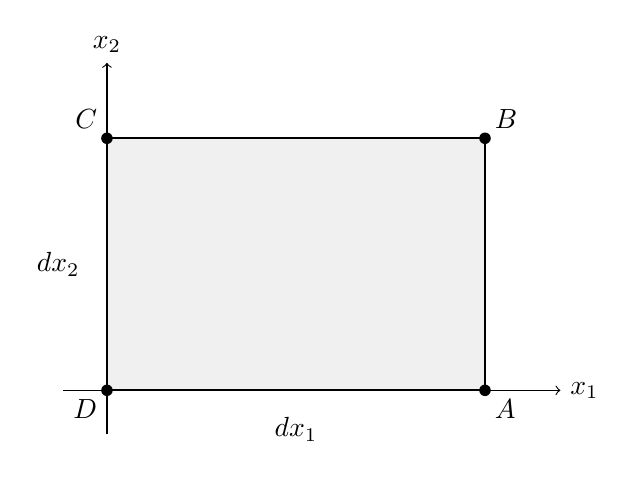
\begin{tikzpicture}[scale=1.6]
  % 坐标轴（矩形位于 x1-x2 平面，法向沿 x3）
  \draw[->] (-0.35,0) -- (3.6,0) node[right]{$x_1$};
  \draw[->] (0,-0.35) -- (0,2.6) node[above]{$x_2$};
  % 矩形：D 在原点，A 在 x1 轴上，C 在纵轴上，B 为右上角
  \coordinate (D) at (0,0);
  \coordinate (A) at (3.0,0);
  \coordinate (B) at (3.0,2.0);
  \coordinate (C) at (0,2.0);
  \fill[gray!12] (D) -- (A) -- (B) -- (C) -- cycle;
  \draw[thick] (D) -- (A) -- (B) -- (C) -- cycle;
  \fill (D) circle (1.3pt) node[below left]{$D$};
  \fill (A) circle (1.3pt) node[below right]{$A$};
  \fill (B) circle (1.3pt) node[above right]{$B$};
  \fill (C) circle (1.3pt) node[above left]{$C$};
  % 边长标注
  \node[below] at (1.5,-0.14) {$dx_1$};
  \node[left] at (-0.14,1.0) {$dx_2$};
\end{tikzpicture}
\par\vspace{2pt}
{\small 图 10.}
\end{figure}

\begin{equation*}
d\ve{S} = dx_1\, dx_2\, \ve{k}.
\end{equation*}

计算(1.52)式右边部分的积分：

\begin{equation*}
\begin{aligned}
\int \nabla \times \ve{A} \cdot d\ve{S}
&= \iint \left(\frac{\partial A_2}{\partial x_1} - \frac{\partial A_1}{\partial x_2}\right) dx_1 dx_2\\
&= \left.\int A_2\, dx_2\right|_{x_1}^{x_1 + dx_1} - \left.\int A_1\, dx_1\right|_{x_2}^{x_2 + dx_2}
\end{aligned}
\end{equation*}

但
\begin{equation*}
\begin{aligned}
\left.\int A_2\right|_{x_1}^{x_1 + dx_1} dx_2 &= \int_{A}^{B} A_2\, dx_2 - \int_{D}^{C} A_2\, dx_2\\
&= \int_{A}^{B} A_2\, dx_2 + \int_{C}^{D} A_2\, dx_2 = \oint A_2\, dx_2.
\end{aligned}
\end{equation*}

另一积分也作相类似的运算后，(1.52)的右边部分即可化成：

\begin{equation}
\iint \left(\frac{\partial A_2}{\partial x_1} - \frac{\partial A_1}{\partial x_2}\right) dx_1 dx_2 = \oint \ve{A} \cdot d\ve{l}.
\tag{1.53}
\end{equation}

这样一来，对于长方形面积元素，定理得证。对于分块光滑的曲面，我们可将它划分为许多个长方形面积元素。应用斯托克斯定理于每一个这种长方形面积元素，并将所得的等式相加，则容易证明斯托克斯定理对于一般情形也是成立的。事实上，两个相邻长方形在邻接边处的各自的走向，正好相反。因此在(1.53)型等式相加时，左边只剩下沿着最外边界（围道 $L$）的曲线积分。

\textbf{附注：}也可对 $n$ 阶张量场作出斯托克斯定理。

今考虑斯托克斯定理在场论中的一些应用。

\textbf{无旋矢量场和位势矢量场。}如果矢量场 $\ve{A}$ 在某个区域 $R$ 内

\begin{equation*}
\nabla \times \ve{A} = 0,
\end{equation*}

则称此场在 $R$ 内是无旋的；如果存在连续标量场 $\Phi$，使在域 $R$ 内处处有

\begin{equation*}
\ve{A} = \nabla\Phi,
\end{equation*}

则称场 $\ve{A}$ 为位势场，而函数 $\Phi$ 称为矢量场 $\ve{A}$ 的位势。

显然，所有位势场都是无旋的，反之则仅对单连通区域才成立。现引进单连通区域的概念。

空间区域 $R$ 称为单连通的，如果位于它里面的任意一条闭曲线 $C$，可以作收缩于一点的连续变形而不超出此区域的范围。

这样，图 11 上的区域 (I) 是平面上的单连通区域，而 (II) 是非单连通区域。在空间中，球、所有凸容积，不仅是整个地，也可以是带有空腔的（例如球带）都可作为单连通区域的例子。而非单连通区域的例子则可举出环面、有空腔的无限圆柱体空间等。

\begin{figure}[htbp]
\centering
\begin{tikzpicture}[scale=1.05]
  % (I) 单连通区域：斜线阴影的圆盘
  \begin{scope}
    \fill[pattern=north east lines, pattern color=gray!50] (0,0) circle (1.3);
    \draw[thick] (0,0) circle (1.3);
    \node at (-1.62,1.32) {Ⅰ};
  \end{scope}
  % (II) 非单连通区域：斜线阴影的圆环
  \begin{scope}[xshift=4.3cm]
    \fill[pattern=north east lines, pattern color=gray!50] (0,0) circle (1.4);
    \fill[white] (0,0) circle (0.6);
    \draw[thick] (0,0) circle (1.4);
    \draw[thick] (0,0) circle (0.6);
    \node at (-1.78,1.42) {Ⅱ};
  \end{scope}
\end{tikzpicture}
\par\vspace{2pt}
{\small 图 11.}
\end{figure}

\begin{figure}[htbp]
\centering
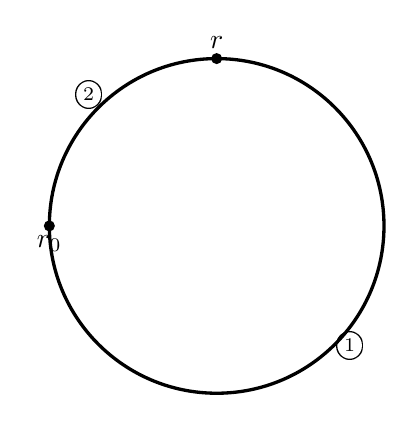
\begin{tikzpicture}[scale=1.25]
  % 闭围道 C（圆），r₀ 在左侧，两条路径 ①、②
  \draw[very thick] (0,0) circle (1.7);
  % 左边缘的点 r₀
  \fill (-1.7,0) circle (1.6pt);
  \node[below] at (-1.7,0) {$r_0$};
  % 顶部点 r
  \fill (0,1.7) circle (1.6pt);
  \node[above] at (0,1.7) {$r$};
  % 路径 ①（右下弧）与 ②（左上弧）
  \node at (1.35,-1.25) {\textcircled{\scriptsize 1}};
  \node at (-1.3,1.3) {\textcircled{\scriptsize 2}};
\end{tikzpicture}
\par\vspace{2pt}
{\small 图 12.}
\end{figure}

在单连通区域内，于每个闭曲线 $C$ 上都可张上整个都在此区域内的分块光滑曲面。

\textbf{定理 1.12}\quad 如果 $R$ 是单连通区域，且在 $R$ 内处处有 $\nabla \times \ve{A} = 0$，则矢量场 $\ve{A}$ 为位势场。即存在 $\Phi$，使 $\nabla\Phi = \ve{A}$。

\textbf{证明}\quad 在 $R$ 内取点 $\ve{r}_0$，置

\begin{equation*}
\Phi(\ve{r}) \equiv \int_{\ve{r}_0}^{\ve{r}} \ve{A} \cdot d\ve{l}
\end{equation*}

（沿着任意路径）。于是由斯托克斯定理及等式 $\nabla \times \ve{A} = 0$ 推出

\begin{equation*}
\oint \ve{A} \cdot d\ve{l} = \int_{S} \nabla \times \ve{A} \cdot d\ve{S} = 0.
\end{equation*}

现在显然
\begin{equation*}
\oint \ve{A} \cdot d\ve{l} = 0 = \int_{\text{\textcircled{\scriptsize 1}}\ \ve{r}_0}^{\ve{r}} \ve{A} \cdot d\ve{l} - \int_{\text{\textcircled{\scriptsize 2}}\ \ve{r}_0}^{\ve{r}} \ve{A} \cdot d\ve{l}.
\end{equation*}

所以 $\Phi(\ve{r})$ 仅是 $\ve{r}$ 的函数。再因

\begin{equation*}
\frac{d}{dx} \int_{0}^{x} f(y)\, dy = f(x),
\end{equation*}

故容易断定
\begin{equation*}
\ve{A} = \nabla\Phi.
\end{equation*}

显然，用矢量场 $\ve{A}$ 确定的标量场 $\Phi$，可精确到一常数被加项，因为

\begin{equation*}
\ve{A} = \nabla\Phi_1 = \nabla\Phi_2, \qquad \Phi_1 - \Phi_2 = \text{const}.
\end{equation*}

\textbf{附注：}区域 $R$ 必须是单连通的。否则 $\oint \ve{A} \cdot d\ve{l}$ 不等于 0。例如，沿着图 13 上的路径且在孔内 $\nabla \times \ve{A} \neq 0$ 的话。不过多连通域可以单连通化。如图 14 所画的那样将它剪开，则带斜线的区域就是单连通的了。但一般说来，这里已经是 $\Phi_{+} \neq \Phi_{-}$，其中

\begin{equation*}
\Phi_{+}(\ve{r}) = \int_{\ve{r}}^{\ve{a}} \ve{A} \cdot d\ve{l}, \qquad \Phi_{-}(\ve{r}) = \int_{\ve{r}}^{\ve{b}} \ve{A} \cdot d\ve{l}.
\end{equation*}

（参看图 14）。因此，无旋矢量场 $\ve{A}$ 在整个区域 $R$ 内不是位势场，因在位势场内函数 $\Phi$ 必须是单值的。如果一场在 $R$ 内的每一点的邻域内都可构造一函数 $\Phi$（局部位势），则称此场为局部位势场。但函数 $\Phi$ 在全域内不再是单值的（多值位势）。

\begin{figure}[htbp]
\centering
\begin{tikzpicture}[scale=1.2]
  % 圆环区域 r₀ < r < R：斜线阴影，三个同心圆
  \fill[pattern=north east lines, pattern color=gray!55] (0,0) circle (1.95);
  \fill[white] (0,0) circle (0.55);
  \draw[thick] (0,0) circle (1.95);
  \draw[thick] (0,0) circle (0.55);
  \draw[thick] (0,0) circle (1.2);
  % 顺时针旋转箭头（左上、右下），标注 r₀ 与 r
  \draw[->,thick] (0,0) ++(165:1.42) arc[start angle=165, delta angle=-60, radius=1.42];
  \node[above left] at (-0.85,1.35) {$r_0$};
  \draw[->,thick] (0,0) ++(330:1.42) arc[start angle=330, delta angle=-60, radius=1.42];
  \node[below right] at (1.05,-1.5) {$r$};
\end{tikzpicture}
\par\vspace{2pt}
{\small 图 13.}
\end{figure}

\begin{figure}[htbp]
\centering
\begin{tikzpicture}[scale=1.15]
  % 外边界：哑铃形（左侧凸起较小，右侧凸起较大，光滑曲线）
  \def\peanut{(-2.7,0) (-2.5,0.55) (-2.1,0.95) (-1.55,1.1) (-0.95,0.98)
              (-0.4,0.78) (0.0,0.62) (0.5,0.95) (1.1,1.35) (1.8,1.5)
              (2.45,1.35) (2.85,0.9) (2.95,0.2) (2.9,-0.35) (2.6,-0.95)
              (2.0,-1.35) (1.3,-1.45) (0.7,-1.25) (0.1,-0.9) (-0.35,-0.7)
              (-0.95,-0.9) (-1.6,-1.05) (-2.2,-0.9) (-2.55,-0.5)}
  \fill[pattern=north east lines, pattern color=gray!55] plot[smooth cycle] coordinates {\peanut};
  % 孔（内边界，近似椭圆，偏右下方）
  \fill[white] (0.85,-0.25) ellipse (0.55 and 0.42);
  % 割线通道（从左侧边界到孔，略带弧度）
  \fill[white] (-2.7,-0.16) rectangle (0.35,0.16);
  % 边界线
  \draw[very thick] plot[smooth cycle] coordinates {\peanut};
  \draw[very thick] (0.85,-0.25) ellipse (0.55 and 0.42);
  % 割线上下缘（略带弧度、向右端略收拢）
  \draw[very thick] (-2.6,0.16) to[bend right=14] (0.32,0.12);
  \draw[very thick] (-2.6,-0.16) to[bend left=14] (0.32,-0.12);
  % 标注：Φ₁ Φ₂、a、b、r
  \node at (-1.5,0.42) {$\Phi_1$};
  \node at (-1.5,-0.42) {$\Phi_2$};
  \node[above right] at (0.32,0.12) {$b$};
  \node[below right] at (0.32,-0.12) {$a$};
  \node at (1.7,0.1) {$r$};
\end{tikzpicture}
\par\vspace{2pt}
{\small 图 14.}
\end{figure}

\textbf{例 15}\quad 静磁学。静磁学方程为

\begin{equation*}
\nabla \times \ve{H} = \frac{4\pi}{c}\, \ve{j},
\end{equation*}

这里 $\ve{H}$ 为磁场矢量，$\ve{j}$ 为流密度。如果在容积 $V$ 内 $\ve{j} \neq 0$，在 $V$ 外 $\ve{j} = 0$，则场 $\ve{H}$ 在 $V$ 外将是无旋的。那么场 $\ve{H}$ 是否是位势场？

如果容积 $V$ 有界，则在 $V$ 外

\begin{equation*}
\ve{H} = \nabla\Phi;
\end{equation*}

如果容积 $V$ 是无界的（流量管），则矢量场 $\ve{H}$ 是非位势的（局部位势）。

% ============================================================
\section{亥姆霍兹定理．麦克斯韦方程}

现在我们叙述并证明一个重要定理。此定理给出了将任一矢量场表示成某个标量函数 $\Phi$ 的梯度与某个散度为零的矢量函数 $\ve{A}$ 的旋度之和。

\textbf{定理 1.13}〔亥姆霍兹（Helmholtz）定理〕\quad 在全空间 $R$ 内单值、连续、有界的矢量场 $\ve{F}$，可分解成位势矢量场和无旋矢量场之和。即可表示为

\begin{equation}
\ve{F} = -\nabla\Phi + \nabla \times \ve{A}, \qquad \text{同时} \quad \nabla \cdot \ve{A} = 0
\tag{1.54}
\end{equation}

标量函数 $\Phi$ 称为矢量场 $\ve{F}$ 的标量位势，而矢量函数 $\ve{A}$ 称为场 $\ve{F}$ 的矢量位势。

\textbf{证明}\quad 定理的证明归结为对所给场 $\ve{F}$，构造满足等式(1.54)的位势 $\Phi$ 和 $\ve{A}$。证明分三步进行。先对两个特殊情形证明定理，尔后推广所得定理于一般情形。

\textbf{1.}\quad 假定所给的矢量场 $\ve{F}$ 满足条件

\begin{equation}
|\ve{F}| < \frac{k}{r^{2+\eta}}, \qquad \eta > 0 \quad (\text{当 } r \to \infty \text{ 时}).
\tag{1.55}
\end{equation}

考虑函数
\begin{equation*}
\ve{G}(\ve{r}) \equiv \int_{\tau} \frac{\ve{F}(\ve{r}')\, d\tau'}{|\ve{r} - \ve{r}'|}.
\end{equation*}

由于所加的条件，此积分收敛，且函数 $\ve{G}(\ve{r})$ 可单值地确定。其次容易验证等式

\begin{equation*}
\nabla^{2}\ve{G}(\ve{r}) = -4\pi\, \ve{F}(\ve{r}).
\end{equation*}

应用(1.33)式于矢量函数 $\ve{G}(\ve{r})$，

\begin{equation*}
\nabla^{2}\ve{G}(\ve{r}) = \nabla[\nabla \cdot \ve{G}(\ve{r})] - \nabla \times [\nabla \times \ve{G}(\ve{r})].
\end{equation*}

现在利用所得的公式，可将函数 $\ve{F}$ 写成

\begin{equation*}
\begin{aligned}
\ve{F} &= -\frac{1}{4\pi} [\nabla(\nabla \cdot \ve{G}) - \nabla \times (\nabla \times \ve{G})]\\
&= -\nabla\Phi + \nabla \times \ve{A},
\end{aligned}
\end{equation*}

式中
\begin{equation*}
\Phi(\ve{r}) = \frac{1}{4\pi}\, \nabla \cdot \ve{G},
\end{equation*}

\begin{equation*}
\ve{A}(\ve{r}) = \frac{1}{4\pi}\, \nabla \times \ve{G}.
\end{equation*}

换言之，在条件(1.55)下，定理得证。若利用函数 $|\ve{r} - \ve{r}'|$ 的对称性，则可将位势 $\Phi$ 和 $\ve{A}$ 表示成更简单的形式。为此，变换 $\nabla_{\ve{r}} \cdot \ve{G}(\ve{r})$ 和 $\nabla_{\ve{r}} \times \ve{G}(\ve{r})$：

\begin{equation*}
\begin{aligned}
\nabla_{\ve{r}} \cdot \ve{G}(\ve{r}) &= \int \nabla_{\ve{r}} \cdot \left(\frac{\ve{F}(\ve{r}')}{|\ve{r} - \ve{r}'|}\right) d\tau'\\
&= \int \ve{F}(\ve{r}') \cdot \nabla_{\ve{r}} \left(\frac{1}{|\ve{r} - \ve{r}'|}\right) d\tau'.
\end{aligned}
\end{equation*}

因
\begin{equation*}
\frac{\partial}{\partial x_i} f(\ve{r} - \ve{r}') = -\frac{\partial}{\partial x_i'}\, f(\ve{r} - \ve{r}'),
\end{equation*}

故有
\begin{equation*}
\nabla_{\ve{r}} \cdot \ve{G}(\ve{r}) = -\int \nabla_{\ve{r}'} \cdot \left(\frac{\ve{F}(\ve{r}')}{|\ve{r} - \ve{r}'|}\right) d\tau' + \int \frac{\nabla_{\ve{r}'} \cdot \ve{F}(\ve{r}')}{|\ve{r} - \ve{r}'|}\, d\tau',
\end{equation*}

应用高斯-奥斯特洛格拉德斯基定理于右边第一个积分，得

\begin{equation*}
\int \nabla_{\ve{r}'} \cdot \left(\frac{\ve{F}(\ve{r}')}{|\ve{r} - \ve{r}'|}\right) d\tau' = \oint \frac{\ve{F}(\ve{r}')}{|\ve{r} - \ve{r}'|} \cdot d\ve{S}',
\end{equation*}

这里对 $d\ve{S}'$ 的积分区域取在半径充分大的球面上。根据条件(1.55)，

\begin{equation*}
\oint \frac{\ve{F}(\ve{r}')}{|\ve{r} - \ve{r}'|} \cdot d\ve{S}' = 0.
\end{equation*}

于是最后有
\begin{equation*}
\nabla_{\ve{r}} \cdot \ve{G}(\ve{r}) = \int \frac{\nabla_{\ve{r}'} \cdot \ve{F}(\ve{r}')}{|\ve{r} - \ve{r}'|}\, d\tau'.
\end{equation*}

其次计算 $\nabla_{\ve{r}} \times \ve{G}(\ve{r})$，有

\begin{equation*}
\begin{aligned}
\nabla_{\ve{r}} \times \ve{G}(\ve{r}) &= \int \nabla_{\ve{r}} \times \left(\frac{\ve{F}(\ve{r}')}{|\ve{r} - \ve{r}'|}\right) d\tau'\\
&= \int \nabla_{\ve{r}} \left(\frac{1}{|\ve{r} - \ve{r}'|}\right) \times \ve{F}(\ve{r}')\, d\tau',
\end{aligned}
\end{equation*}

或
\begin{equation*}
\begin{aligned}
\nabla_{\ve{r}} \times \ve{G}(\ve{r}) &= -\int \nabla_{\ve{r}'} \times \left\{\frac{\ve{F}(\ve{r}')}{|\ve{r} - \ve{r}'|}\right\} d\tau'\\
&\qquad + \int \nabla_{\ve{r}'} \times \ve{F}(\ve{r}') \frac{d\tau'}{|\ve{r} - \ve{r}'|}.
\end{aligned}
\end{equation*}

由高斯-奥斯特洛格拉德斯基定理及条件(1.55)可推出对 $d\tau'$ 的第一个积分为零。这样一来，

\begin{equation*}
\nabla_{\ve{r}} \times \ve{G}(\ve{r}) = \int \frac{\nabla_{\ve{r}'} \times \ve{F}(\ve{r}')}{|\ve{r} - \ve{r}'|}\, d\tau'.
\end{equation*}

为了将所得结果表示成更紧凑的形式，我们引进量 $\rho$ 和 $\ve{j}$。置

\begin{equation*}
\nabla \cdot \ve{F} = 4\pi\rho, \qquad \nabla \times \ve{F} = 4\pi\ve{j},
\end{equation*}

则
\begin{equation}
\Phi(\ve{r}) = \int \frac{\rho(\ve{r}')}{|\ve{r} - \ve{r}'|}\, d\tau',
\tag{1.56}
\end{equation}

\begin{equation}
\ve{A}(\ve{r}) = \int \frac{\ve{j}(\ve{r}')}{|\ve{r} - \ve{r}'|}\, d\tau'.
\tag{1.57}
\end{equation}

必须注意，标量位势和矢量位势的获得，归结为求解如下的标量方程和矢量方程：

\begin{equation}
-\nabla^{2}\Phi = 4\pi\rho,
\tag{1.58a}
\end{equation}

\begin{equation}
-\nabla^{2}\ve{A} = 4\pi\ve{j}.
\tag{1.58b}
\end{equation}

方程(1.58a)、(1.58b)分别称为标量和矢量的泊松方程。当它们相应的齐次方程，即拉普拉斯方程只有零解时，它们才有唯一解。显然，标量和矢量位势分别可精确到一调和函数（拉普拉斯方程的解）和它的梯度。由定理的证明过程推出的调和函数的一个性质是很有趣的。

\textbf{推论}\quad 如果函数 $\Phi$ 满足拉普拉斯方程 $\nabla^{2}\Phi = 0$，而在无穷远处为

\begin{equation*}
\frac{1}{r^{1+\eta}} \qquad (\text{当 } |\ve{r}| \to \infty,\ \eta > 0),
\end{equation*}

则它恒等于零。

\textbf{证明}\quad 用等式 $\ve{F} = -\nabla\Phi$ 确定一矢量场 $\ve{F}$，则

\begin{equation*}
4\pi\ve{j} = \nabla \times \ve{F} = 0, \qquad 4\pi\rho = \nabla \cdot \ve{F} = -\nabla^{2}\Phi = 0.
\end{equation*}

因有条件：
\begin{equation*}
\Phi \longrightarrow \frac{1}{|\ve{r}|^{1+\eta}},
\end{equation*}

故当 $|\ve{r}| \to \infty$ 时

\begin{equation*}
|\nabla\Phi| \longrightarrow \frac{1}{r^{2+\eta}}.
\end{equation*}

因此由亥姆霍兹定理推出 $\Phi = 0$。

\textbf{2.}\quad 现研究矢量场的旋度满足下面条件时的情形：

\begin{equation}
\text{当 } r \to \infty \text{ 时，} \nabla \times \ve{F} \text{ 与 } \frac{1}{|\ve{r}|^{2+\eta}} \text{ 同级。}
\tag{1.59}
\end{equation}

设矢量位势 $\ve{A}$ 如前面(1.57)式那样给出。为了证明定理，只须先检验是否满足等式(1.54)，然后再指出 $\nabla \cdot \ve{A} = 0$。先证 $\nabla \cdot \ve{A} = 0$。计算 $\nabla \cdot \ve{A}$，有

\begin{equation*}
\begin{aligned}
\nabla \cdot \ve{A} &= \int \nabla_{\ve{r}} \cdot \left(\frac{\ve{j}(\ve{r}')}{|\ve{r} - \ve{r}'|}\right) d\tau'\\
&= \int \frac{\nabla_{\ve{r}'} \cdot \ve{j}(\ve{r}')}{|\ve{r} - \ve{r}'|}\, d\tau' - \int \nabla_{\ve{r}'} \cdot \left(\frac{\ve{j}(\ve{r}')}{|\ve{r} - \ve{r}'|}\right) d\tau';
\end{aligned}
\end{equation*}

但
\begin{equation*}
\ve{j} = \frac{1}{4\pi}\, \nabla \times \ve{F},
\end{equation*}

因 $\nabla \cdot \ve{j} = 0$，故第一个积分等于零。第二个积分根据高斯-奥斯特洛格拉德斯基定理进行变换，并利用条件(1.59)，有

\begin{equation*}
\int \nabla_{\ve{r}'} \cdot \left(\frac{\ve{j}(\ve{r}')}{|\ve{r} - \ve{r}'|}\right) d\tau' = \int \ve{j}(\ve{r}') \cdot \frac{d\ve{S}'}{|\ve{r} - \ve{r}'|} \longrightarrow \frac{|\ve{r}|^{2}}{|\ve{r}|^{3+\eta}}.
\end{equation*}

根据前面的证明推出，它也等于零。这样一来，矢量场 $\ve{A}$ 是无散的。

等式(1.54)的正确性是不难检验的。为此，利用关系式(1.33)。即可得

\begin{equation*}
\nabla \times (\nabla \times \ve{A}) = 4\pi\ve{j}.
\end{equation*}

因此对任意矢量 $\ve{A}$ 和 $\ve{F}$，有

\begin{equation*}
\nabla \times (\ve{F} - \nabla \times \ve{A}) = 0.
\end{equation*}

这就推出了等式(1.54)。

\textbf{3.}\quad 现对 $\ve{F}$ 不加任何附加的限制。为了在这种一般场合证明定理，考虑半径为 $R$ 的球，并引进记号

\begin{equation*}
\ve{Q}(\ve{r}) =
\begin{cases}
\ve{F}(\ve{r}), & \text{当 } |\ve{r}| < R \text{ 时},\\
0, & \text{当 } |\ve{r}| > R \text{ 时};
\end{cases}
\end{equation*}

\begin{equation*}
\ve{J}(\ve{r}) =
\begin{cases}
\ve{j}(\ve{r}) = \dfrac{1}{4\pi}\, \nabla \times \ve{F}, & \text{当 } |\ve{r}| < R \text{ 时},\\
0, & \text{当 } |\ve{r}| > R \text{ 时};
\end{cases}
\end{equation*}

现证此时 $\nabla \cdot \ve{A} = 0$，这里：

\begin{equation*}
\ve{A} = \int \frac{1}{|\ve{r} - \ve{r}'|}\, \ve{J}(\ve{r}')\, d\tau'
\end{equation*}

\begin{equation*}
\begin{aligned}
\nabla_{\ve{r}} \cdot \ve{A} &= \int \nabla_{\ve{r}} \cdot \left(\frac{1}{|\ve{r} - \ve{r}'|}\right) \ve{J}(\ve{r}')\, d\tau'\\
&= -\int \nabla_{\ve{r}'} \cdot \left[\frac{\ve{J}(\ve{r}')}{|\ve{r} - \ve{r}'|}\right] d\tau' + \int \frac{\nabla_{\ve{r}'} \cdot \ve{J}(\ve{r}')}{|\ve{r} - \ve{r}'|}\, d\tau'.
\end{aligned}
\end{equation*}

第一个积分等于零，此因它可归结为充分大半径 $R$ 的球面上的曲面积分。而由关系式

\begin{equation*}
\ve{J}(\ve{r}) = \frac{1}{4\pi}\, \nabla \times \ve{Q}(\ve{r}),
\end{equation*}

推出 $\nabla \cdot \ve{J} = 0$，故第二个积分也等于零。因此 $\nabla \cdot \ve{A} = 0$ 得证，而(1.54)式对 $\ve{Q}(\ve{r})$ 的正确性无需特别检验。因此在半径为 $R$ 的球所包围的区域内有：

\begin{equation*}
\ve{F} = \nabla \times \ve{A} - \nabla\Phi \qquad (\nabla \cdot \ve{A} = 0).
\end{equation*}

将球半径趋向于无穷大，就知定理在空间的任一有限部分都成立。这就完全证明了定理。

\textbf{例 16}\quad 利用标量位势和矢量位势来表示电磁场。大家知道，电磁场完全可用矢量 $\ve{E}$ 和 $\ve{H}$（电场和磁场强度矢量）来描述。建立这些量之间的联系的麦克斯韦方程，是实验物理定律的概括。今研究这些方程。

\textbf{1.} $\nabla \cdot \ve{E} = 4\pi\rho$。此方程表示，电荷是静电场的源。它也可从库仑定律导出。

\textbf{2.} $\nabla \cdot \ve{H} = 0$。此方程断定，磁荷是不存在的，它也可从磁力线的封闭性得出。

\textbf{3.} 麦克斯韦第三方程

\begin{equation*}
\nabla \times \ve{H} = \frac{4\pi}{c}\, \ve{j} + \frac{1}{c}\, \frac{\partial\ve{E}}{\partial t}
\end{equation*}

推广了比奥-萨伐尔（Biot--Savart）定律。

\textbf{4.} 最后，第四方程

\begin{equation*}
\nabla \times \ve{E} = -\frac{1}{c}\, \frac{\partial\ve{H}}{\partial t}
\end{equation*}

表达了法拉第电磁感应定律。显然，从麦克斯韦方程组寻求电磁场的问题需要计算构成矢量 $\ve{E}$ 和 $\ve{H}$ 的六个分量。不过它可归结为仅找四个量，即标量位势 $\Phi$ 和三个构成矢量位势 $\ve{A}$ 的分量。

因用矢量位势 $\ve{A}$ 确定的 $\ve{H} = \nabla \times \ve{A}$，有 $\nabla \cdot \ve{H} = 0$。故由麦克斯韦方程组可推出下面这些关系式：

由麦克斯韦第四方程得

\begin{equation*}
\nabla \times \left(\ve{E} + \frac{1}{c}\, \dot{\ve{A}}\right) = 0,
\end{equation*}

即
\begin{equation*}
\ve{E} + \frac{1}{c}\, \dot{\ve{A}} = -\nabla\Phi;
\end{equation*}

由第一方程得：

\begin{equation*}
\nabla \cdot \left(-\nabla\Phi - \frac{1}{c}\, \dot{\ve{A}}\right) = 4\pi\rho,
\end{equation*}

或
\begin{equation*}
-\nabla^{2}\Phi - \frac{1}{c}\, \nabla \cdot \dot{\ve{A}} = 4\pi\rho;
\end{equation*}

由第三方程得：

\begin{equation*}
\nabla \times (\nabla \times \ve{A}) - \frac{1}{c}\, \frac{\partial}{\partial t}\left(-\nabla\Phi - \frac{1}{c}\, \dot{\ve{A}}\right) = \frac{4\pi}{c}\, \ve{j},
\end{equation*}

或
\begin{equation*}
-\nabla^{2}\ve{A} + \frac{1}{c^{2}}\, \ddot{\ve{A}} + \nabla\left(\nabla \cdot \ve{A} + \frac{1}{c}\, \dot{\Phi}\right) = \frac{4\pi}{c}\, \ve{j}.
\end{equation*}

因为 $\nabla \cdot \ve{A}$ 是任意的，故可这样选取 $\ve{A}$，使

\begin{equation*}
\nabla \cdot \ve{A} + \frac{1}{c}\, \dot{\Phi} = 0
\end{equation*}

[这个等式称为洛伦兹（Lorentz）条件]。于是

\begin{equation*}
\ve{E} = -\nabla\Phi - \frac{1}{c}\, \dot{\ve{A}}, \qquad \ve{H} = \nabla \times \ve{A}.
\end{equation*}

而函数 $\Phi$ 与 $\ve{A}$ 满足下面的方程

\begin{equation}
\nabla^{2}\Phi - \frac{1}{c^{2}}\, \ddot{\Phi} = -4\pi\rho,
\tag{1.60}
\end{equation}

\begin{equation*}
\nabla^{2}\ve{A} - \frac{1}{c^{2}}\, \ddot{\ve{A}} = -\frac{4\pi}{c}\, \ve{j}.
\end{equation*}

如果场不依赖于时间（静力学的情形），我们就得到 $\ve{A}$ 和 $\Phi$ 的泊松（拉普拉斯）数量或矢量方程。

记
\begin{equation*}
\nabla^{2} - \frac{1}{c^{2}}\, \frac{\partial^{2}}{\partial t^{2}} \equiv \square^{2},
\end{equation*}

算子 $\square^{2}$ 称为达朗贝尔（D'Alembert）算子。利用算子 $\square^{2}$，方程(1.60)可简写为

\begin{equation}
\begin{aligned}
\square^{2}\Phi &= -4\pi\rho,\\
\square^{2}\ve{A} &= -\frac{4\pi}{c}\, \ve{j}.
\end{aligned}
\tag{1.60a}
\end{equation}

考虑齐次情形 $(\rho = 0,\ \ve{j} = 0)$。则

\begin{equation}
\square^{2}\psi = 0, \qquad \text{这里 } \psi = \{\Phi, A_1, A_2, A_3\}
\tag{1.61}
\end{equation}

方程(1.61)的特解为：

\begin{equation*}
\psi = f(z), \qquad z = t - \frac{\ve{u} \cdot \ve{r}}{c},
\end{equation*}

这里 $\ve{u}$ 为任意方向上的单位矢量，$f$ 为坐标的任意函数。这个结论可由下列计算得到证明：

\begin{equation*}
\begin{aligned}
\frac{\partial\psi}{\partial x_i} &= \frac{\partial f}{\partial z}\, \frac{\partial z}{\partial x_i} = -\frac{u_i}{c}\, \frac{df}{dz},\\
\frac{\partial^{2}\psi}{\partial x_i^{2}} &= -\frac{u_i}{c}\, \frac{d^{2}f}{dz^{2}}\, \frac{dz}{dx_i} = \frac{u_i^{2}}{c^{2}}\, \frac{d^{2}f}{dz^{2}},\\
\frac{\partial\psi}{\partial t} &= \frac{df}{dz}, \qquad \frac{\partial^{2}\psi}{\partial t^{2}} = \frac{d^{2}f}{dz^{2}};
\end{aligned}
\end{equation*}

由此（注意到 $u_1^{2} + u_2^{2} + u_3^{2} = 1$，即 $\ve{u}$ 为单位矢量）：

\begin{equation}
\square^{2}\psi = \sum_{i=1}^{3} \left(\frac{u_i^{2}}{c^{2}} - \frac{1}{c^{2}}\right) \frac{d^{2}f}{dz^{2}} = 0.
\tag{1.61a}
\end{equation}

方程(1.61)是线性的，即对于它迭加原理成立，即：如果 $\psi_1$ 和 $\psi_2$ 是它的解，则它们的和 $\psi_1 + \psi_2$ 也是它的解。因此，我们可指望方程(1.61)的通解具有下面的形状：

\begin{equation*}
\psi = \sum_{i} f_i \left(t - \ve{u}_i \cdot \frac{\ve{r}}{c}\right).
\end{equation*}

解的物理意义是容易明白的，这只需考虑它随时间变化的性态。设

\begin{equation*}
\psi = \psi_0 \sin(\ve{k} \cdot \ve{r} - \omega t),
\end{equation*}

这里
\begin{equation*}
c = \frac{\omega}{k},
\end{equation*}

\begin{equation*}
\ve{k} \cdot \ve{r} - \omega t = \omega \left(\frac{\ve{k}}{\omega} \cdot \ve{r} - t\right) = \omega \left(\frac{\ve{u} \cdot \ve{r}}{c} - t\right).
\end{equation*}

在任一固定点，经过与周期 $T = \frac{2\pi}{\omega}$ 相等的时间间隔后，它的图象又重现。在任一瞬间距曲线上给定点的距离为 $\lambda = \frac{2\pi}{|\ve{k}|}$ 的地方，图象又重复。这里 $\lambda$ 为波长，$\omega$ 为圆频率，$k$ 为波数（在距离 $2\pi$ 之内的波的数目）。

% ============================================================
\section{曲线坐标系中的基本微分运算}

在某些问题中，空间中点的位置不用三维笛卡尔坐标 $(x, y, z)$ 而用被称为点的曲线坐标 $(\xi_1, \xi_2, \xi_3)$ 来确定是比较方便的。此时

\begin{equation*}
\begin{aligned}
x &= \varphi_1(\xi_1, \xi_2, \xi_3), \quad y = \varphi_2(\xi_1, \xi_2, \xi_3), \quad z = \varphi_3(\xi_1, \xi_2, \xi_3);\\
\xi_1 &= \psi_1(x, y, z), \quad \xi_2 = \psi_2(x, y, z), \quad \xi_3 = \psi_3(x, y, z).
\end{aligned}
\end{equation*}

在研究这种坐标系时，引进坐标曲面，即曲面 $\xi_i = \text{const}$ 及其交线，是很有用的。

如果在空间中的任一点处的三条坐标曲线相互正交，换句话说，三条坐标曲线的单位切向矢量相互垂直，则此曲线坐标系就称为正交曲线坐标系。

坐标系正交的条件可写成

\begin{equation}
\frac{\partial\varphi_1}{\partial\xi_i}\, \frac{\partial\varphi_1}{\partial\xi_k}
+ \frac{\partial\varphi_2}{\partial\xi_i}\, \frac{\partial\varphi_2}{\partial\xi_k}
+ \frac{\partial\varphi_3}{\partial\xi_i}\, \frac{\partial\varphi_3}{\partial\xi_k} = 0 \qquad (i \neq k)
\tag{1.62}
\end{equation}

而在坐标 $(\xi_1, \xi_2, \xi_3)$ 处的长度元素，利用上式即可表示成

\begin{equation*}
\begin{aligned}
dS^{2} &= dx^{2} + dy^{2} + dz^{2}\\
&= \left(\frac{\partial\varphi_1}{\partial\xi_1}\, d\xi_1 + \frac{\partial\varphi_1}{\partial\xi_2}\, d\xi_2 + \frac{\partial\varphi_1}{\partial\xi_3}\, d\xi_3\right)^{2}\\
&\qquad + \left(\frac{\partial\varphi_2}{\partial\xi_1}\, d\xi_1 + \frac{\partial\varphi_2}{\partial\xi_2}\, d\xi_2 + \frac{\partial\varphi_2}{\partial\xi_3}\, d\xi_3\right)^{2}\\
&\qquad + \left(\frac{\partial\varphi_3}{\partial\xi_1}\, d\xi_1 + \frac{\partial\varphi_3}{\partial\xi_2}\, d\xi_2 + \frac{\partial\varphi_3}{\partial\xi_3}\, d\xi_3\right)^{2}\\
&= h_1^{2}\, d\xi_1^{2} + h_2^{2}\, d\xi_2^{2} + h_3^{2}\, d\xi_3^{2}.
\end{aligned}
\end{equation*}

这里
\begin{equation*}
h_i = \sqrt{\left(\frac{\partial\varphi_1}{\partial\xi_i}\right)^{2} + \left(\frac{\partial\varphi_2}{\partial\xi_i}\right)^{2} + \left(\frac{\partial\varphi_3}{\partial\xi_i}\right)^{2}}.
\end{equation*}

量 $h_i$ 称为（给定坐标系的）拉梅（Lam\'e）参数。

\textbf{例 17}\quad 球坐标。在这种坐标系中，点的位置用三个参数 $r$，$\theta$，$\varphi$ 来确定（图 15）。

\begin{equation*}
\begin{aligned}
x &= r \sin\theta \cos\varphi, \qquad y = r \sin\theta \sin\varphi, \qquad z = r \cos\theta;\\
dS^{2} &= dr^{2} + r^{2}\, d\theta^{2} + r^{2} \sin^{2}\theta\, d\varphi^{2},\\
h_1 &= 1, \qquad h_2 = r, \qquad h_3 = r \sin\theta.
\end{aligned}
\end{equation*}

柱面坐标（图 16）。

\begin{figure}[htbp]
\centering
\begin{tikzpicture}[tdplot_main_coords, scale=2.4]
  \coordinate (O) at (0,0,0);
  % 坐标轴
  \draw[->,thick] (O) -- (2.0,0,0) node[anchor=north east]{$x$};
  \draw[->,thick] (O) -- (0,2.0,0) node[anchor=north west]{$y$};
  \draw[->,thick] (O) -- (0,0,1.9) node[anchor=south]{$z$};
  % 矢径 r 及其端点
  \coordinate (P) at (1.15,0.85,1.15);
  \coordinate (Pxy) at (1.15,0.85,0);
  \draw[->,very thick] (O) -- (P) node[midway,right]{$r$};
  % 虚线投影框架（长方体轮廓）
  \draw[dashed] (P) -- (0,0,1.15);        % 端点到 z 轴（水平）
  \draw[dashed] (P) -- (Pxy);             % 端点到 xy 平面（竖直）
  \draw[dashed] (O) -- (Pxy);             % 原点 → 投影点
  \draw[dashed] (Pxy) -- (1.15,0,0);      % 投影点 → x 轴
  \draw[dashed] (Pxy) -- (0,0.85,0);      % 投影点 → y 轴
  \draw[dashed] (0,0,1.15) -- (0,0.85,0);
  \fill (P) circle (1.2pt);
  % φ 弧（x 轴与 xy 平面内投影线之间）
  \draw[->,thick] plot[domain=0:36.5, samples=14] ({0.55*cos(\x)},{0.55*sin(\x)},{0});
  \node at (0.72,0.30,0) {$\varphi$};
  % θ 弧（z 轴与 r 之间）
  \draw[->,thick] plot[domain=0:51.2, samples=16]
    ({0.6*sin(\x)*0.6267},{0.6*sin(\x)*0.4632},{0.6*cos(\x)+0.6*sin(\x)*0.6267});
  \node at (0.42,0.42,0.30) {$\theta$};
\end{tikzpicture}
\par\vspace{2pt}
{\small 图 15.}
\end{figure}

\begin{figure}[htbp]
\centering
\begin{tikzpicture}[tdplot_main_coords, scale=2.3]
  \coordinate (O) at (0,0,0);
  % 坐标轴
  \draw[->,thick] (O) -- (2.0,0,0) node[anchor=north east]{$x$};
  \draw[->,thick] (O) -- (0,2.0,0) node[anchor=north west]{$y$};
  \draw[->,thick] (O) -- (0,0,1.9) node[anchor=south]{$z$};
  % 位置矢量 r、投影 ρ（原书为黑白）
  \coordinate (P) at (1.15,0.85,1.15);
  \coordinate (Rho) at (1.15,0.85,0);
  \draw[->,very thick] (O) -- (P) node[midway,right]{$r$};
  \draw[very thick] (O) -- (Rho) node[pos=0.68,below=7pt]{$\rho$};
  % 虚线：P 竖直向下到 ρ 末端；P 水平向左到 z 轴
  \draw[dashed] (P) -- (Rho) node[midway,right]{$z$};
  \draw[dashed] (P) -- (0,0,1.15);
  % φ 弧（x 与 ρ 之间）
  \draw[->,thick] plot[domain=0:36.5, samples=14] ({0.55*cos(\x)},{0.55*sin(\x)},{0});
  \node at (0.72,0.30,0) {$\varphi$};
  \fill (P) circle (1.2pt);
\end{tikzpicture}
\par\vspace{2pt}
{\small 图 16.}
\end{figure}

\begin{equation*}
\begin{aligned}
\xi_1 &= \rho, \qquad \xi_2 = \varphi, \qquad \xi_3 = z.\\
x &= \rho \cos\varphi, \qquad y = \rho \sin\varphi, \qquad z = z,\\
dS^{2} &= d\rho^{2} + \rho^{2}\, d\varphi^{2} + dz^{2},\\
h_1 &= 1, \qquad h_2 = \rho, \qquad h_3 = 1.
\end{aligned}
\end{equation*}

表达式
\begin{equation*}
\ve{A}(\ve{r}) \cdot \ve{e}_i(\ve{r})
\end{equation*}

称为在曲线坐标系中矢量 $\ve{A}$ 的坐标。这里 $\ve{e}_i$ 为在坐标曲线

\begin{equation*}
\xi_j = \text{const}, \qquad \xi_k = \text{const}, \qquad j \neq k \neq i
\end{equation*}

方向上的单位矢量。显然，标量函数 $\Phi$ 的梯度在曲线坐标系中等于

\begin{equation*}
(\nabla\Phi)_i = (\nabla\Phi \cdot \ve{e}_i) = \frac{\partial\Phi}{h_i\, \partial\xi_i} = \frac{1}{h_i}\, \frac{\partial\Phi}{\partial\xi_i}.
\end{equation*}

现求散度与旋度的表达式。因为构成矢量 $\ve{e}_i$ 的笛卡尔坐标从一点变到另一点时将会改变，所以在微分时必须小心。我们避免这个困难，而利用基于高斯-奥斯特洛格拉德斯基定理和斯托克斯定理的散度、旋度定义的不变性。对于散度有

\begin{equation*}
\nabla \cdot \ve{A} = \lim_{\triangle v \to 0} \frac{1}{\triangle v} \oint \ve{A} \cdot d\ve{S}.
\end{equation*}

应用这个公式于体积元素 $\triangle v$（图 17），并计算经过相互面对着的两个边界面 $ABCD$ 和 $EFGH$ 上的流量差：

\begin{figure}[htbp]
\centering
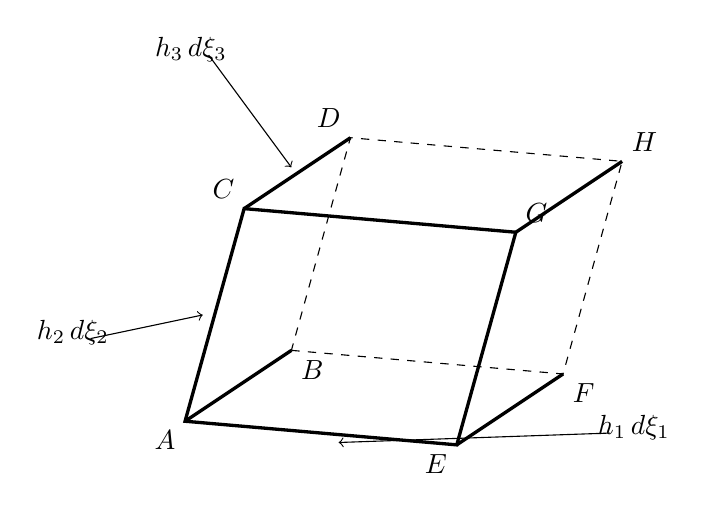
\begin{tikzpicture}[scale=1.5]
  % 曲面六面体：前面 A-E-G-C（实线），后面 B-F-H-D（虚线），深度棱 A-B、E-F、G-H、C-D（实线）
  \coordinate (A) at (1.3,0.6);
  \coordinate (E) at (3.6,0.4);
  \coordinate (G) at (4.1,2.2);
  \coordinate (C) at (1.8,2.4);
  \coordinate (B) at (2.2,1.2);
  \coordinate (F) at (4.5,1.0);
  \coordinate (H) at (5.0,2.8);
  \coordinate (D) at (2.7,3.0);
  % 背面（虚线）
  \draw[dashed] (B) -- (F) -- (H) -- (D) -- cycle;
  % 前面（实线）
  \draw[very thick] (A) -- (E) -- (G) -- (C) -- cycle;
  % 深度棱（实线）
  \draw[very thick] (A) -- (B) (E) -- (F) (G) -- (H) (C) -- (D);
  % 顶点标注
  \node[below left]  at (A) {$A$};
  \node[below left]  at (E) {$E$};
  \node[above right] at (G) {$G$};
  \node[above left]  at (C) {$C$};
  \node[below right] at (B) {$B$};
  \node[below right] at (F) {$F$};
  \node[above right] at (H) {$H$};
  \node[above left]  at (D) {$D$};
  % 拉梅系数标注（带引线箭头）
  \draw[->] (4.9,0.5) -- (2.6,0.42);
  \node at (5.1,0.55) {$h_1\, d\xi_1$};
  \draw[->] (0.5,1.3) -- (1.45,1.5);
  \node at (0.35,1.35) {$h_2\, d\xi_2$};
  \draw[->] (1.5,3.7) -- (2.2,2.75);
  \node at (1.35,3.75) {$h_3\, d\xi_3$};
\end{tikzpicture}
\par\vspace{2pt}
{\small 图 17.}
\end{figure}

\begin{figure}[htbp]
\centering
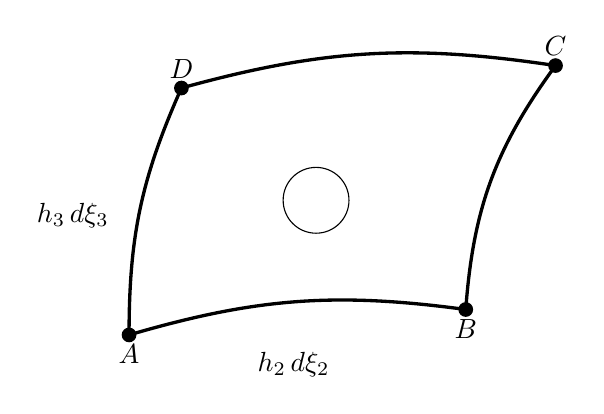
\begin{tikzpicture}[scale=1.9]
  % 曲边四边形 ABCD（ξ2ξ3 面）
  \coordinate (A) at (0.35,0.45);
  \coordinate (B) at (2.6,0.62);
  \coordinate (C) at (3.2,2.25);
  \coordinate (D) at (0.7,2.1);
  \draw[very thick] (A) to[bend left=12] (B) to[bend left=16] (C) to[bend right=12] (D) to[bend right=12] (A);
  \fill (A) circle (1.4pt) node[below]{$A$};
  \fill (B) circle (1.4pt) node[below]{$B$};
  \fill (C) circle (1.4pt) node[above]{$C$};
  \fill (D) circle (1.4pt) node[above]{$D$};
  % 线元标注
  \node[below] at (1.45,0.4) {$h_2\, d\xi_2$};
  \node[left] at (0.28,1.25) {$h_3\, d\xi_3$};
  % 内部空心圆
  \draw (1.6,1.35) circle (0.22);
\end{tikzpicture}
\par\vspace{2pt}
{\small 图 18.}
\end{figure}

\begin{equation*}
Q_1 = \frac{\partial}{\partial\xi_1} (A_1 h_2 h_3)\, d\xi_1\, d\xi_2\, d\xi_3.
\end{equation*}

类似地计算经过另外界面的流量差：

\begin{equation*}
Q_2 = \frac{\partial}{\partial\xi_2} (A_2 h_3 h_1)\, d\xi_1\, d\xi_2\, d\xi_3,
\end{equation*}

\begin{equation*}
Q_3 = \frac{\partial}{\partial\xi_3} (A_3 h_1 h_2)\, d\xi_1\, d\xi_2\, d\xi_3.
\end{equation*}

由此得到最后的结果：

\begin{equation*}
\nabla \cdot \ve{A} = \frac{1}{h_1 h_2 h_3} \left[ \frac{\partial}{\partial\xi_1} (h_2 h_3 A_1) + \frac{\partial}{\partial\xi_2} (h_1 h_3 A_2) + \frac{\partial}{\partial\xi_3} (h_1 h_2 A_3) \right].
\end{equation*}

例如，在球面坐标系中

\begin{equation*}
\operatorname{div}\ve{A} = \frac{1}{r^{2}}\, \frac{\partial (A_r r^{2})}{\partial r} + \frac{1}{r\sin\theta}\, \frac{\partial (A_\theta \sin\theta)}{\partial\theta} + \frac{1}{r\sin\theta}\, \frac{\partial A_\varphi}{\partial\varphi};
\end{equation*}

在柱面坐标系中

\begin{equation*}
\operatorname{div}\ve{A} = \frac{1}{\rho}\, \frac{\partial (\rho A_\rho)}{\partial\rho} + \frac{1}{\rho}\, \frac{\partial A_\varphi}{\partial\varphi} + \frac{\partial A_z}{\partial z}.
\end{equation*}

现考虑 $\operatorname{rot}\ve{A}$，它可用下面的方式确定：

\begin{equation*}
(\nabla \times \ve{A})_i = \lim_{S_i \to 0} \frac{1}{S_i} \oint \ve{A} \cdot d\ve{l}.
\end{equation*}

问题在于计算矢量 $\ve{A}$ 沿着图 18 上的闭围路 $ABCD$ 的环量。它等于四个被加项的代数和：

\begin{equation*}
\begin{aligned}
AB &\longrightarrow A_2 h_2\, d\xi_2 \big|_{\xi_3},\\
CD &\longrightarrow -A_2 h_2\, d\xi_2 \big|_{\xi_3 + d\xi_3},\\
BC &\longrightarrow A_3 h_3\, d\xi_3 \big|_{\xi_2 + d\xi_2},\\
DA &\longrightarrow -A_3 h_3\, d\xi_3 \big|_{\xi_2}.
\end{aligned}
\end{equation*}

因此
\begin{equation*}
\oint \ve{A} \cdot d\ve{l} = \left[-\frac{\partial}{\partial\xi_3} (A_2 h_2) + \frac{\partial}{\partial\xi_2} (A_3 h_3)\right] d\xi_2\, d\xi_3.
\end{equation*}

曲边四边形 $ABCD$ 的面积等于

\begin{equation*}
d\sigma_1 = h_2 h_3\, d\xi_2\, d\xi_3,
\end{equation*}

所以
\begin{equation*}
(\nabla \times \ve{A})_1 = \frac{1}{h_2 h_3} \left[ \frac{\partial}{\partial\xi_2} (A_3 h_3) - \frac{\partial}{\partial\xi_3} (A_2 h_2) \right],
\end{equation*}

类似地有：
\begin{equation*}
(\nabla \times \ve{A})_2 = \frac{1}{h_3 h_1} \left[ \frac{\partial}{\partial\xi_3} (A_1 h_1) - \frac{\partial}{\partial\xi_1} (A_3 h_3) \right],
\end{equation*}

\begin{equation*}
(\nabla \times \ve{A})_3 = \frac{1}{h_1 h_2} \left[ \frac{\partial}{\partial\xi_1} (A_2 h_2) - \frac{\partial}{\partial\xi_2} (A_1 h_1) \right].
\end{equation*}

例如，在球面坐标系中

\begin{equation*}
\operatorname{rot}_r \ve{A} = \frac{1}{r\sin\theta}\, \frac{\partial (A_\varphi \sin\theta)}{\partial\theta} - \frac{1}{r\sin\theta}\, \frac{\partial A_\theta}{\partial\varphi},
\end{equation*}

\begin{equation*}
\operatorname{rot}_\theta \ve{A} = \frac{1}{r\sin\theta}\, \frac{\partial A_r}{\partial\varphi} - \frac{1}{r}\, \frac{\partial (r A_\varphi)}{\partial r},
\end{equation*}

\begin{equation*}
\operatorname{rot}_\varphi \ve{A} = \frac{1}{r}\, \frac{\partial (r A_\theta)}{\partial r} - \frac{1}{r}\, \frac{\partial A_r}{\partial\theta};
\end{equation*}

在柱面坐标系中

\begin{equation*}
\operatorname{rot}_\rho \ve{A} = \frac{1}{\rho}\, \frac{\partial A_z}{\partial\varphi} - \frac{\partial A_\varphi}{\partial z},
\end{equation*}

\begin{equation*}
\operatorname{rot}_\varphi \ve{A} = \frac{\partial A_\rho}{\partial z} - \frac{\partial A_z}{\partial\rho},
\end{equation*}

\begin{equation*}
\operatorname{rot}_z \ve{A} = \frac{1}{\rho}\, \frac{\partial (\rho A_\varphi)}{\partial\rho} - \frac{1}{\rho}\, \frac{\partial A_\rho}{\partial\varphi}.
\end{equation*}
